\documentclass[
  amsfonts,
  amsmath,
  tbtags,
  amssymb,
  aps,
  nobibnotes,
  %% prl,
  twocolumn,
  superscriptaddress,
]{revtex4-2}

% imports
\usepackage{appendix}[titletoc]
\usepackage[english]{babel}
\usepackage[justification=centering]{caption}
\usepackage{float}
\usepackage{graphicx}
\usepackage{hyperref}
\usepackage[utf8]{inputenc}
\usepackage{layouts}
\usepackage{optidef}
\usepackage{physics}
\usepackage{setspace}
\usepackage[labelformat=simple]{subcaption}
\usepackage{xcolor}

% configure imports
\DeclareMathOperator*{\argmin}{arg\,min}
\newcommand{\todo}[1]{\textcolor{red}{TODO: #1}}
\definecolor{darkgreen}{RGB}{46, 184, 46}
\newcommand{\half}{\frac{1}{2}}
\newcommand{\R}{\mathbb{R}}
\captionsetup[subfigure]{labelformat=empty, skip=0pt}
\restylefloat{table}
\renewcommand\thesubfigure{(\alph{subfigure})}



\begin{document}


%% TITLE
\title{Robust Control of a Fluxonium Qubit}

\author{Thomas Propson}
\email{tcpropson@uchicago.edu}
\affiliation{
  James Franck Institute, University of Chicago, Chicago, Illinois 60637, USA
}
\affiliation{
  Department of Physics, University of Chicago, Chicago, Illinois 60637, USA
}
\author{Brian Jackson}
\author{Zac Manchester}
\affiliation{
  Department of Aeronautics and Astronautics Engineering, Stanford University, 496 Lomita Mall, Stanford, CA 94305
}
\author{David I. Schuster}
\affiliation{
  James Franck Institute, University of Chicago, Chicago, Illinois 60637, USA
}
\affiliation{
  Department of Physics, University of Chicago, Chicago, Illinois 60637, USA
}
\affiliation{
  Pritzker School of Molecular Engineering, University of Chicago, Chicago, Illinois 60637, USA
}

\date{\today}


%% ABSTRACT
\begin{abstract}
  %% - 1 + 2 topic importance
  %% - 1 what I have done
  %% - few sentences about primary results
  The ability to engineer high fidelity operations on quantum processors in the presence of
  calibration errors and decoherence remains the primary challenge requisite to achieving quantum advantage.
  Quantum optimal control (QOC) techniques have proven effective in realizing high fidelity operations,
  but they require exquisite calibration to be performant. In this work we employ robust trajectory optimization techniques
  to achieve high fidelity gates for parameter spreads on the order of $1\%$. 
  Additionally, current QOC techniques mitigate decoherence effects due to longitudinal relaxation by integrating
  the Lindblad master equation, which increases the computational complexity
  of the optimization algorithm.
  In this work we achieve a factor of $5$ increase in longitudinal relaxation times
  for the gate set of a fluxonium qubit
  using a computationally efficient metric in optimizaiton.
\end{abstract}

\maketitle


%% S1
\section{Introduction}
textwidth: \printinunitsof{in}\prntlen{\textwidth}
linewidth: \printinunitsof{in}\prntlen{\linewidth}
%% P1 - general field, lots of citation. cite reviews, original qoc.
%% P2 - exhaustively find all papers, what people have done to address the issues
%% P3 - what we do is. maybe add a rant about how
%% QOC is classical control theory but we've ignored that field
%% P4 - outline
(The field) The field of quantum optimal control (QOC) is concerned
with efficiently and accurately manipulating quantum systems.
Early QOC techniques were proposed for nuclear magnetic resonance experiments
\cite{khaneja2005optimal}, and applications now include superconducting
qubits \cite{heeres2017implementing,
  leng2019robust, leung2017speedup, xu2020nonadiabatic},
neutral and ionized atoms \cite{van2016optimal}, nitrogen-vacancy centers in
diamond \cite{rembold2020introduction}, and Bose-Einstien condensates
\cite{sorensen2018quantum}.
In quantum control theory, as in classical control theory,
optimization is performed
to minimize an objective function. Relevant for the field
of quantum computation is the task of achieving high fidelity quantum gates.
In this application, the objective function includes contributions from the
gate error associated with the state transfer of the system as well as contributions
due to experimental constraints, such as the control amplitude.
The decision variables of the optimization problem are the time-dependent control
parameters, particular to the quantum system, that govern its evolution.

(Existing work) Many analytic and numerical techniques have been developed to control
quantum systems. Analytic methods rely on solving the time-dependent
Schroedinger equation analytically or deriving equations of motion
from a suitable Lagrangian \cite{zhang2020universal, huang2020engineering, han2020experimental,
  xu2020nonadiabatic, carlini2005quantum}. Analytic methods
have been presented to address decoherence in quantum systems.
Considering the dynamical and geometric phases of state
evolution has led to methods for achieving
robustness to dynamical errors and mitigating pure dephasing
\cite{xu2020nonadiabatic, han2020experimental, merrill2014progress}.
Additionally, suitable choices of bases have been proposed that
allow the experimentalist to infer tradeoffs in longitudinal relaxation
and pure dephasing coherence times \cite{huang2020engineering}.
To date, however, no analytical method has been presented
to construct a gate while satisfying arbitrary experimental
constraints. Furthermore, most analytic methods have only
been demonstrated in the two-level approximation and become
cumbersome to solve for larger Hilbert space sizes.


Numerical quantum control techniques have developed in parallel
with analytic frameworks.
Most numerical techniques proposed for QOC are indirect shooting
methods where an initial guess for the control trajectory is forward-simulated,
e.g. under the time-dependent Schroedinger equation,
and first-order gradients are computed for a functional evaluated
on the state of the evolved system \cite{leung2017speedup,  goerz2019krotov, doria2011optimal,
  abdelhafez2019gradient, machnes2015gradient, leng2019robust}.
Most techniques formulate the
problem as unconstrained or use
projective gradient methods to enforce constraints
\cite{machnes2015gradient}.
The latter approach relies on constructing
bases for constraint spaces--which is not always feasible--and
may hinder convergence.
Methods for mitigating decoherence using numerical
techniques have employed master equation dynamics (citation needed),
Monte Carlo style trajectories \cite{abdelhafez2019gradient},
and proposals have been made to simulate multiple trajectories
\cite{reinhold2019controlling, rembold2020introduction}.

(This work) In this work, we employ state of the art
trajectory optimization methods
to formulate the quantum
optimal control problem as a constrained optimization problem, allowing
us to enforce arbitrary experimental constraints.
Additionally,
we introduce methods for constructing gates that mitigate longitudinal
relaxation and are robust to experimental errors, and therefore
pure dephasing, the dominant barriers to experimentally
realizing practical quantum computing.

(Outline) As an example, we study the quantum optimal control problem on
the fluxonium qubit presented in \cite{zhang2020universal}.
We describe experimentally realistic constraints and map them to
the trajectory optimization framework. Next, we
outline a method for making the optimization longitudinal
relaxation aware. We achieve a factor of 5 increase in longitudinal relaxation times
over the baseline gate set.
We present two methods for achieving robustness to pure dephasing
and compare them to existing dynamic decoupling methods. We find that
the methods we employ are able to produce high fidelity gates when
subject to parameter spreads of $1\%$.


%% S2
\section{QOC + AL-iLQR}
(QOC Problem Statement) Here we introduce the notation
we will use throughout the paper,
review the quantum optimal control problem statement,
and introduce the trajectory optimization framework.
Quantum optimal control concerns the evolution of
a quantum state $\ket{\psi(t)}$ governed by the time-dependent
Schroedinger equation (TDSE)
\label{eq:tdse}
\begin{align}
  \frac{d}{dt} \ket{\psi(t)} &= -\frac{i}{\hbar} H(u(t), t) \ket{\psi(t)}
\end{align}
The evolution is sometimes cast with the evolution
of a density matrix under the Lindblad master equation to
model the decoherence of the state explicitly. The Hamiltonian
has an arbitrary dependence on the possibly multi-valued controls $u(t)$.
The controls are so called because they are the means the experimentalist has to
act on the system.

Numerical quantum optimal control techniques make
the problem tractable by discretizing the problem into $N$
knot points (time steps). Typical integration techniques for the TDSE include
approximating unitary propagators as well as explicit integration methods,
such as Runge-Kutta, of the form
$\ket{\psi_{k + 1}} \approx \ket{\psi_{k}} + \frac{d}{dt} \ket{\psi_{k}} \cdot \Delta t_{k}$

Quantum optimal control seeks the control
parameters that minimize a functional $J(u(t))$.
In the simplest case the functional is
$J = 1 - {\lvert \braket{\psi_{f} \lvert \psi_{N}(u(t))} \rvert}^{2}$
the infidelity between the inital state evolved
to the final knot point ($\ket{\psi_{N}(u(t))}$)
and the target state ($\ket{\psi_{f}}$). In general
$J$ is a linear combinaion of cost functions on the state, e.g.
forbidden-state occupation, as well as
cost functions on the controls, e.g. the norm of the control amplitudes
\cite{leung2017speedup}. Typical quantum optimal control
algorithms employ automatic differentiation
to compute first order information for the functional ($\nabla_{u} J(u)$).
They employ a first-order optimizer to minimize $J$ with respect to $u$.

(AL-iLQR Problem Statement) The trajectory optimization
literature solves a more general class of non-linear programs that resemble
the quantum optimal control problem. The quantum optimal control
problem is a specific case of the linear quadratic regulator (LQR).
LQR is so called because the dynamics are linear in the state and
the functional is quadratic in the state. In the LQR formulation
the same functional is evaluated at each knot point
\begin{equation}
  J_{\textrm{iLQR}} = \tilde{x}_{N}^{T} Q_{N} \tilde{x}_{N}
  + \sum_{k = 0}^{N - 1} \tilde{x}_{k}^{T} Q_{k} \tilde{x}_{k} + u_{k}^{T} R_{k} u_{k}
\end{equation}
where $\tilde{x}_{k} = x_{k} - x_{f}$ is the difference between the state
at knot point $k$ and final state, $u_{k}$ are the controls,
and $Q_{k}, R_{k}$ are matrices that define the penalty metric.
The state is propagated using a dynamics function
$x_{k + 1} = f(x_{k}, u_{k}, t_{k}, \Delta t_{k})$.
In the case of quantum optimal control $\ket{\psi_{k}} \subseteq x_{k}$
and $f$ encodes the TDSE dynamics. In the following
we refer to $\ket{\psi}$ as the state. We refer to $x$ and $u$ as
the augmented state and augmented controls, respectively.

The advantage of the LQR formulation
is that there exists a dynamic programming algorithm to compute the
optimal update to the augmented controls ($u_{k}$) which minimizes the functional
($J_{\textrm{iLQR}, k}$) for each knot point. This algorithm proceeds by deriving a
recurrence relation between knot points $k$ and $k + 1$ for the optimal
feedback law--known as the Ricatti recursion (see Appendix). The
iterative LQR (iLQR) algorithm computes $J_{\textrm{iLQR}}$
and applies the Ricatti recursion to all knot points on multiple
executions.

In order to incorporate constraints we employ
the augmented Lagrangian method. Constraints are contributions
to the functional of arbitrary form $c_{k}(x_{k}, u_{k})$ which are
zero or negative when the constraint is satisfied. The AL-iLQR
method associates a penalty multiplier with the functional
that estimates the constraint's Lagrange multiplier.
The algorithm updates the penalty multiplier between
iLQR executions. In this scheme the functional takes the form
\begin{equation}
  \begin{aligned}
    J_{\textrm{AL-iLQR}} = \ &(\lambda_{k} + \frac{1}{2}I_{\mu_{k}} c_{k}(x_{k}, u_{k}))^{T} c_{k}(x_{k}, u_{k})\\
    &+ J_{\textrm{iLQR}}
  \end{aligned}
\end{equation}
where $\lambda_{k}$ is a Lagrange multiplier and $I_{\mu_{k}}$ is a penalty matrix
with $\mu_{k}$ along the diagonal.
$\lambda_{k}$ and $\mu_{k}$ are updated after each augmented Lagrangian iteration according to
\begin{align}
  \lambda_{k_{i}} &\gets \max(0, \lambda_{k_{i}} + \mu_{k_{i}} c_{k_{i}}(x_{k}^{*}, u_{k}^{*}))\\
  \mu_{k_{i}} &\gets \phi \mu_{k_{i}}
\end{align}
where $x^{*}, u^{*}$ are the optimal augmented state and augmented controls from the iLQR execution,
$i$ indicates the $i$-th constraint functional,
and $\phi$ is a hyperparameter. With this updated form of the cost
functional there still exists a recurrence relation to calculate the optimal control
updates, see \cite{howell2019altro}.


%% S3
\section{QOC on the Fluxonium}
(Fluxonium Device) In the following we study
the quantum optimal control problem on the fluxonium qubit.
In the two-level
approximation the system Hamiltonian takes the form
\label{eq:hamiltonian}
\begin{align}
  H/h &= f_{q} \frac{\sigma_{z}}{2} + a(t) \frac{\sigma_{x}}{2}
\end{align}
where $f_{q} = 14$MHz is the qubit frequency at the flux frustration point,
$a$ is the flux drive amplitude, $h$ is Planck's constant, and $\sigma_{x}, \sigma_{y}$
are Pauli matrices. The flux amplitude $a$ is experimentally
realized by modulating the flux 
threading the device. We consider the task of constructing $Z/2$, $Y/2$, and $X/2$
gates for the fluxonium qubit subject to experimental constraints, decoherence, and
system parameter deviations. We compare the gates we obtain with optimal
control methods to the analytically constructed gates reported in
\cite{zhang2020universal} for the same device.
%% The flux amplitude is obtained from the external flux by
%% $a = 4 \pi \braket{g \lvert \hat{\phi} \rvert e} \rvert_{0.5 \Phi_{0}} E_{L}
%% \delta \Phi_{\textrm{ext}} / (h \Phi_{0})$
%% where $\hat{\phi}$ is the phase operator, $E_{L}$ is the characteristic inductance energy, $\Phi_{0}$
%% is a flux quantum, and
%% $\delta \Phi_{\textrm{ext}} = \Phi_{\textrm{ext}} - 0.5 \Phi_{0}$ is the flux
%% offset from the flux frustration point.

(Constraints) We now present the constraints we require each gate
to obey.
To ensures gates may be concatenated arbitrarily without
inducing AWG ringing due to high-frequency transitions,
we require $a(t = 0) = a(t = t_{N}) = 0$.
Furthermore, we require $\int_{0}^{t_{N}} a(t) dt = 0$. This
constraint ensures the pulse has zero net flux, mitigating
the hysteresis ubiquitous in flux bias lines.
%% TODO: See ref. 28 in Helin paper
We require $-0.5 \textrm{GHz} \le a(t) \le 0.5 \textrm{GHz}$
to ensure the two-level approximation \ref{eq:hamiltonian}
remains valid. Additionally, we require that each gate achieves
the desired state transition $\ket{\psi_{N}} = \ket{\psi_{f}}$.
In addition to these constraints we penalize the norm
of the first and second derivatives of the flux amplitude to
ensure its smoothness, and in doing so mitigate AWG ringing.

The optimization is performed over the second derivative of the flux amplitude
$\frac{d^{2}}{dt^{2}} a$ which is contained in the
augmented control vector. The first derivative
$\frac{d}{dt} a$, proportional $a$, and integral $\int a$
flux amplitude terms
are contained in the augmented state vector. They are obtained from
the second derivative of the flux amplitude by
integration in the dynamics function.
Both the zero net flux and target quantum state constraint
are then handled by ensuring the target augmented state is
reached $x_{N} = x_{f}$.
The equality and inequality constraints on $a$ are handled
with a bound constraint.
%% TODO: probably want to list equations for the constraints

($T_{1}$ and $T_{\phi}$ noise)
In addition to constructing gates
that obey experimental constraints and have high simulated fidelities,
we also desire to make the gates robust to noise that affects the experimental
gate fidelity. Decoherence of the quantum state due to external noise
is typically modeled by two phenomena: longitudinal relaxation and pure dephasing.
They are modeled using their $1/e$ decay times $T_{1}$ and $T_{\phi}$ respectively
(see Appendix).
The main contributions to longitudinal relaxation in our
device are dielectric loss in the capacitor, resistive loss in the inductor,
and Purcell loss. The main contributions to pure dephasing in our
device are $1/f$ flux noise and decay via charge and flux coupling
to the control lines.

Dissipation to the thermal bath via longitudinal
relaxation is an irreversible process
that results in information loss.
Converesely, pure dephasing is a reversible process.
There is a tradeoff between the two decoherence processes. In the case of white
noise we have that the sum of the noise weights $W_{1}$ and $W_{\phi}$
is constant \cite{huang2020engineering}.
Our device achieves its best pure dephasing
protection at the flux frustration point
$T_{2e}(a = 0) \sim 300 \mu\textrm{s}$
where the qubit is first-order insensitive to changes in flux.
It becomes more succeptable to pure dephasing as the flux is tuned away from the flux
frustration point $|a| > 0$. Conversely, longitudinal relaxation is at a minimum
at the flux frustration point $T_{1}(a = 0) = 0.315$ms,
and increases away from the flux frustration point
$T_{1}(a = 0.34 \textrm{GHz}) = 4.3$ms. Given the nature
of the decay processes and the tradeoff, we choose
to maximize the longitudinal relaxation time directly
via the flux amplitude and employ robust control techniques to mitigate
pure dephasing.

%% F1
\begin{figure*}[ht]
  \begin{subfigure}{.315\textwidth}
    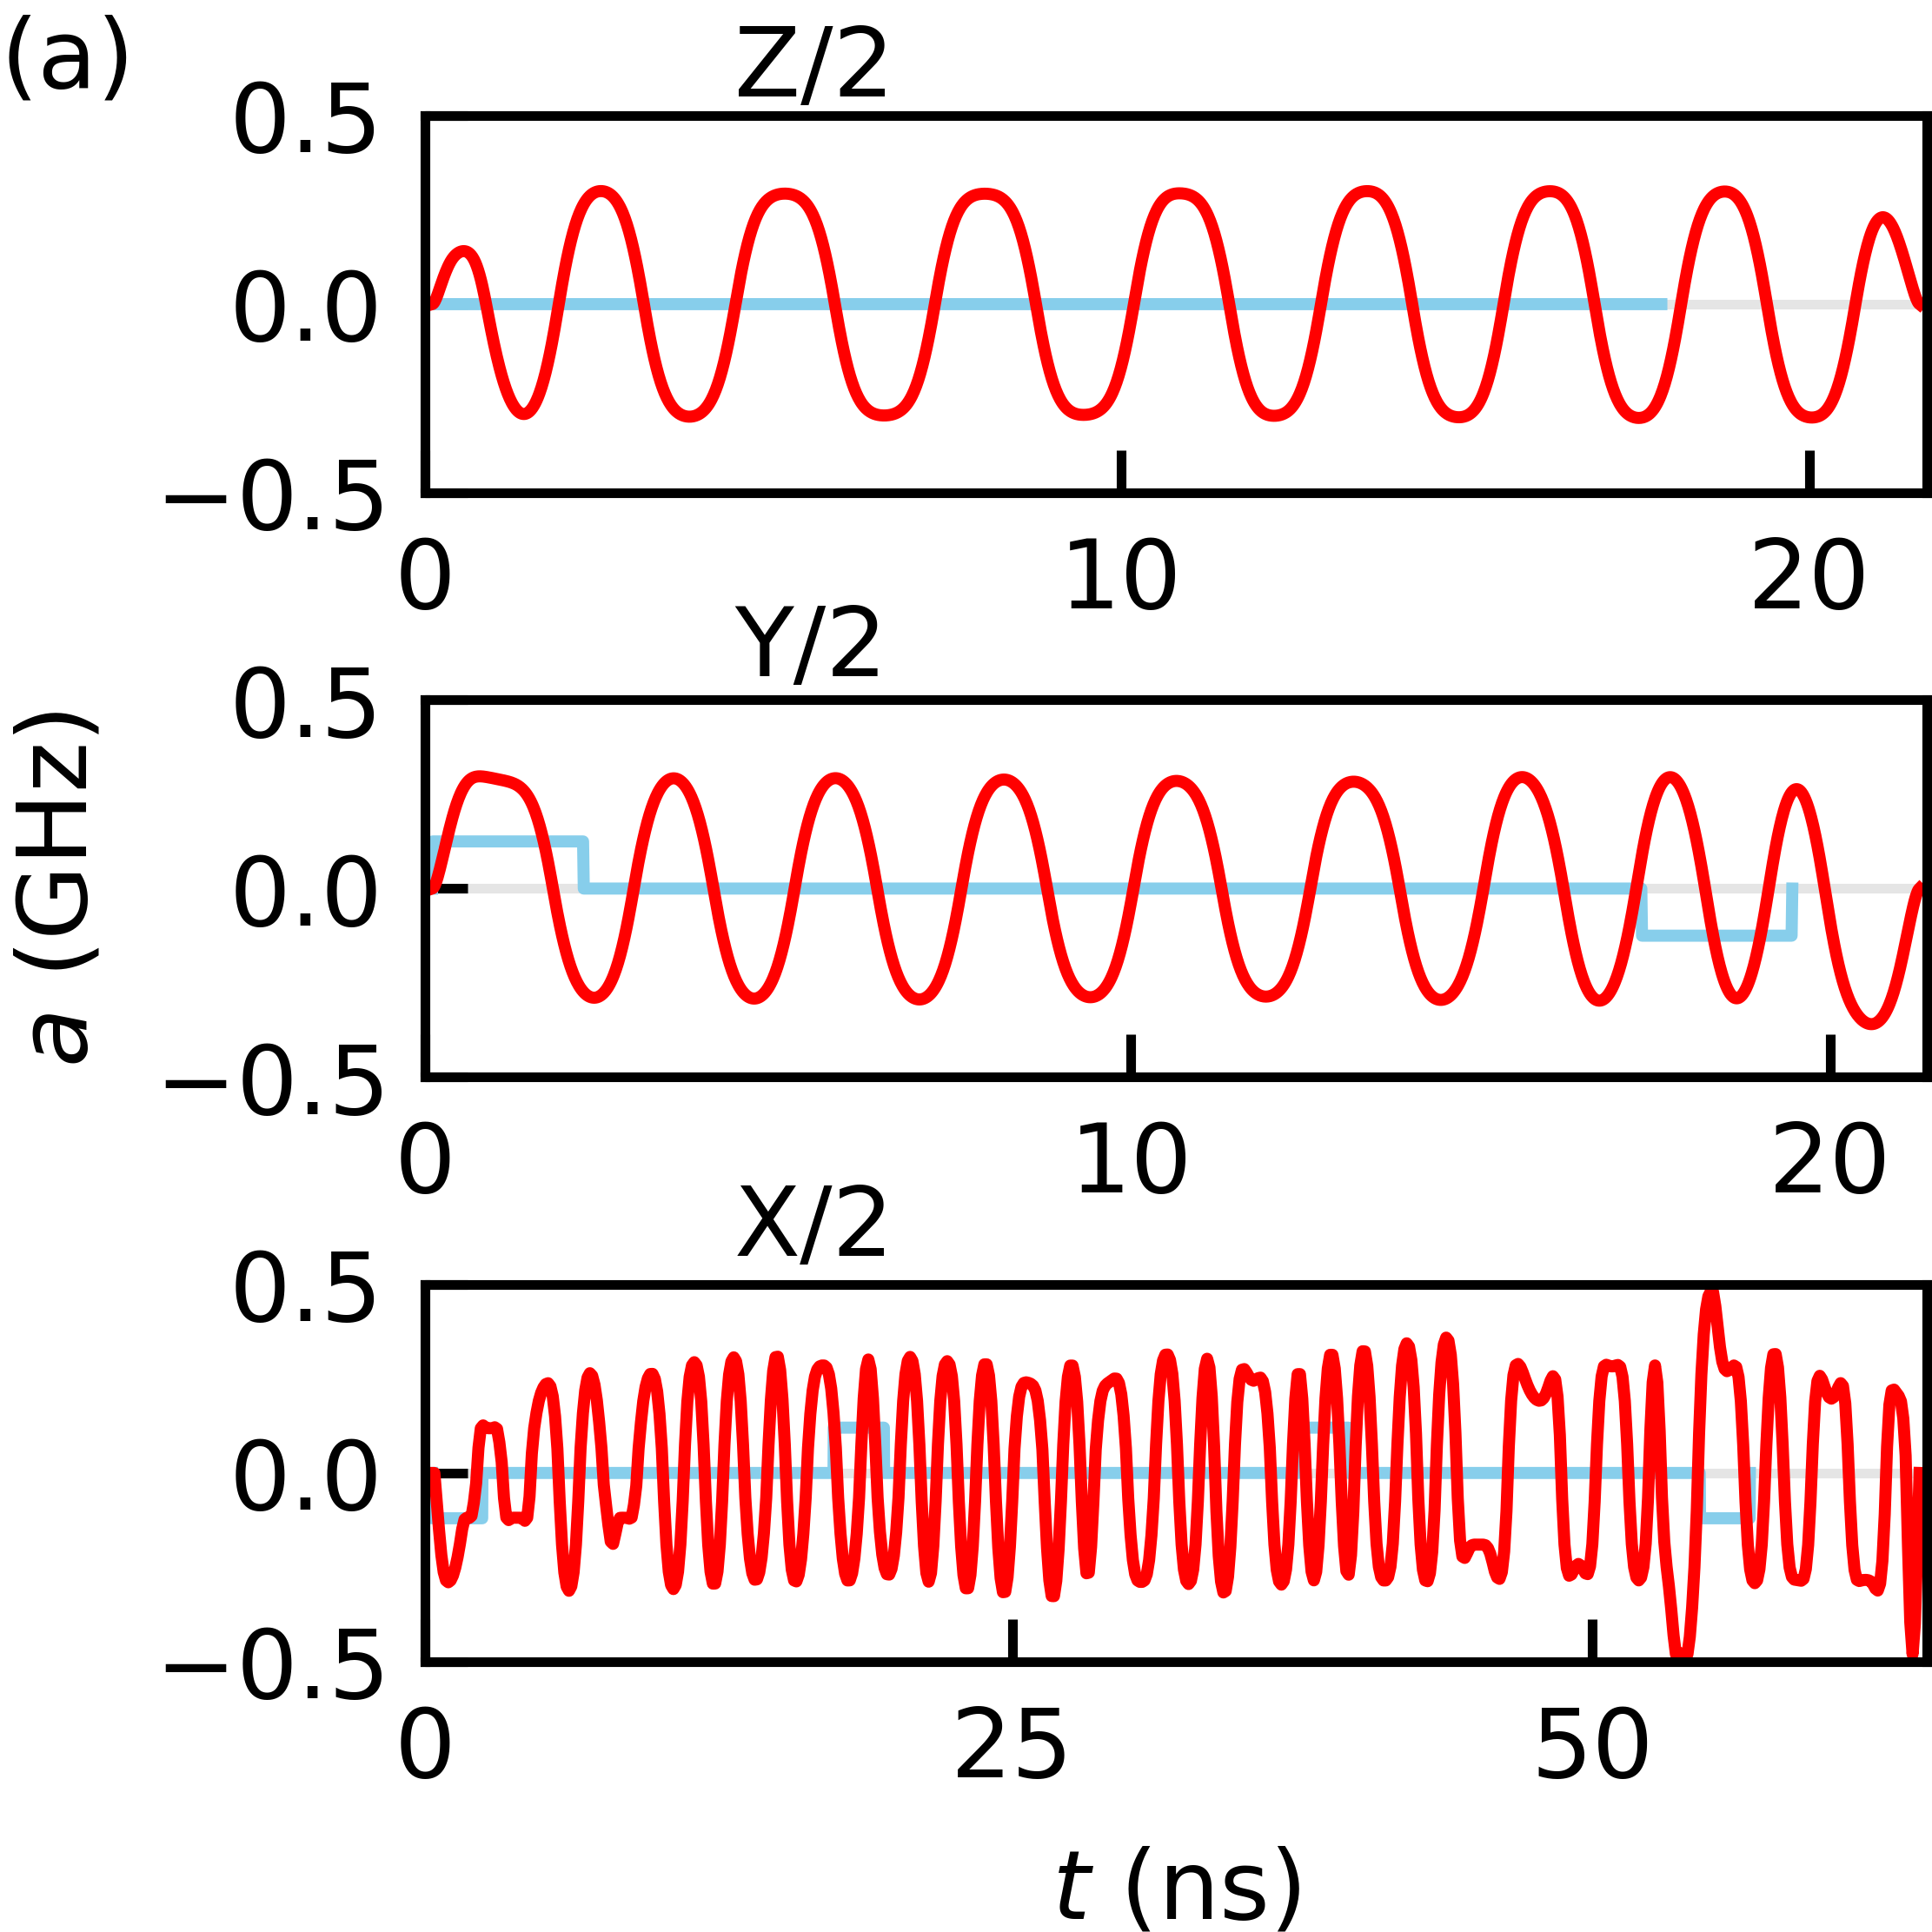
\includegraphics[width=\linewidth]{assets/f1a.png}
  \end{subfigure}\hfill
  \begin{subfigure}{.23\textwidth}
    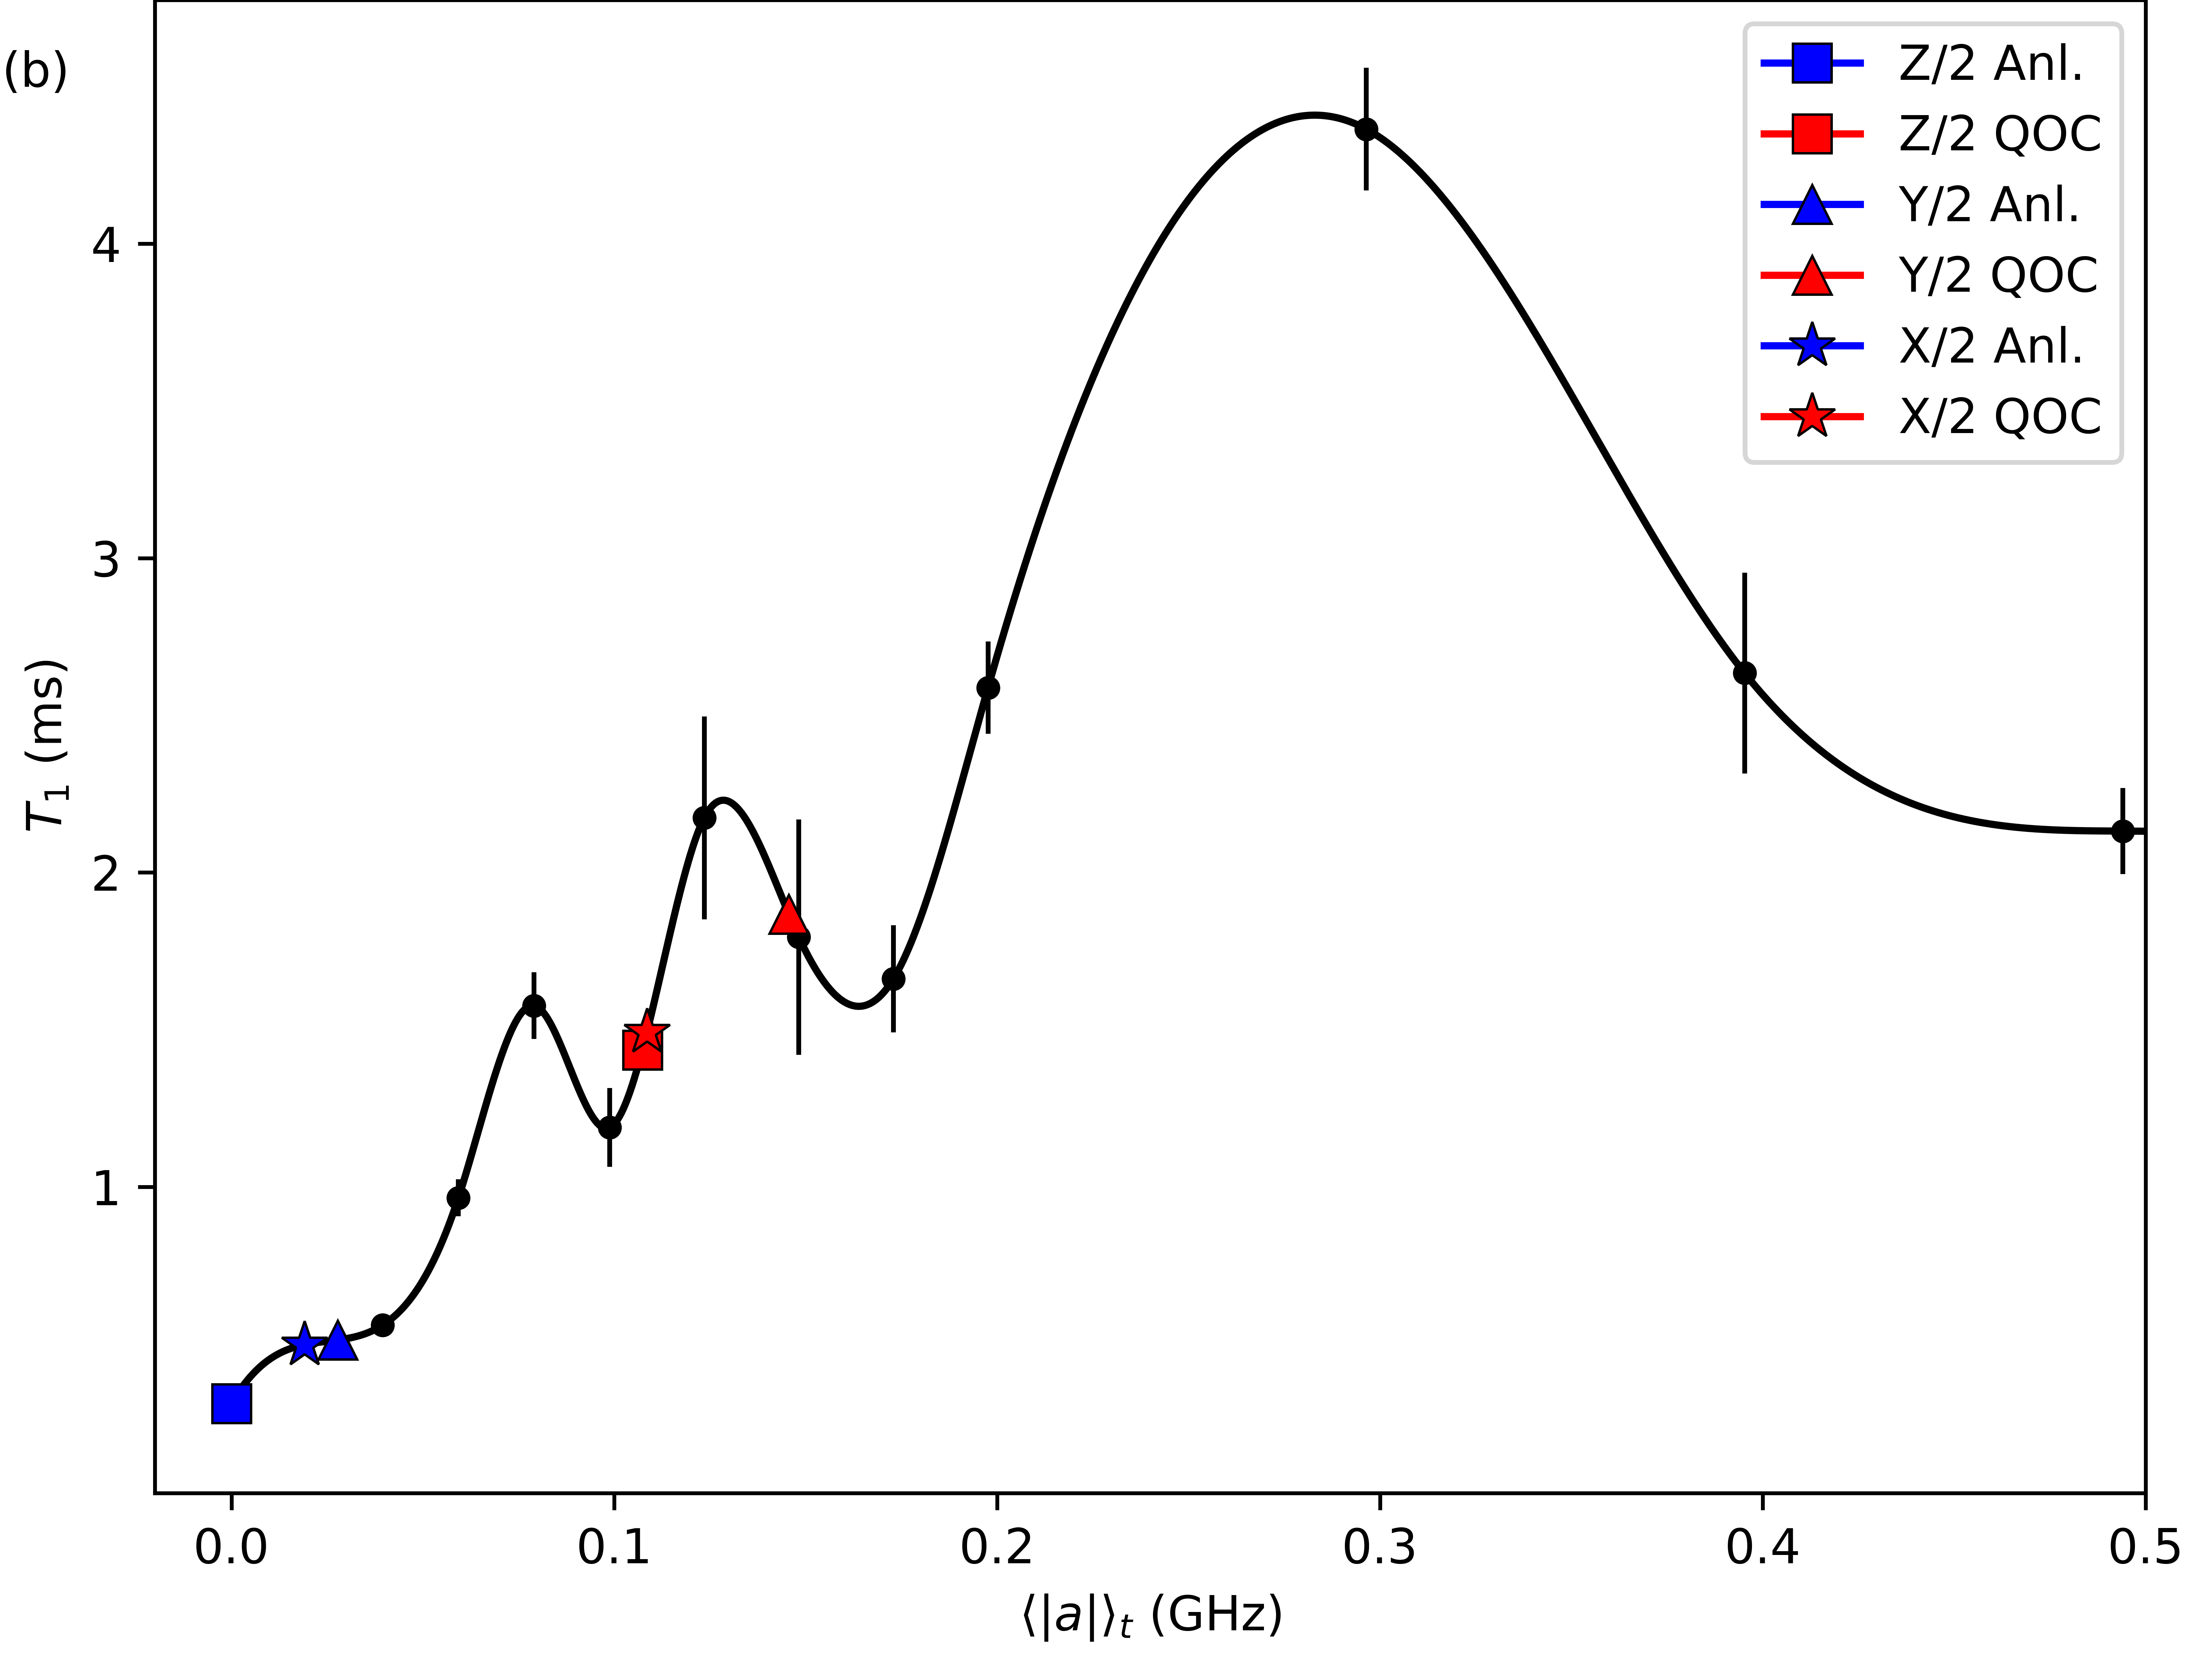
\includegraphics[width=\linewidth]{assets/f1b.png}
  \end{subfigure}\hfill
  \begin{subfigure}{.4\textwidth}
    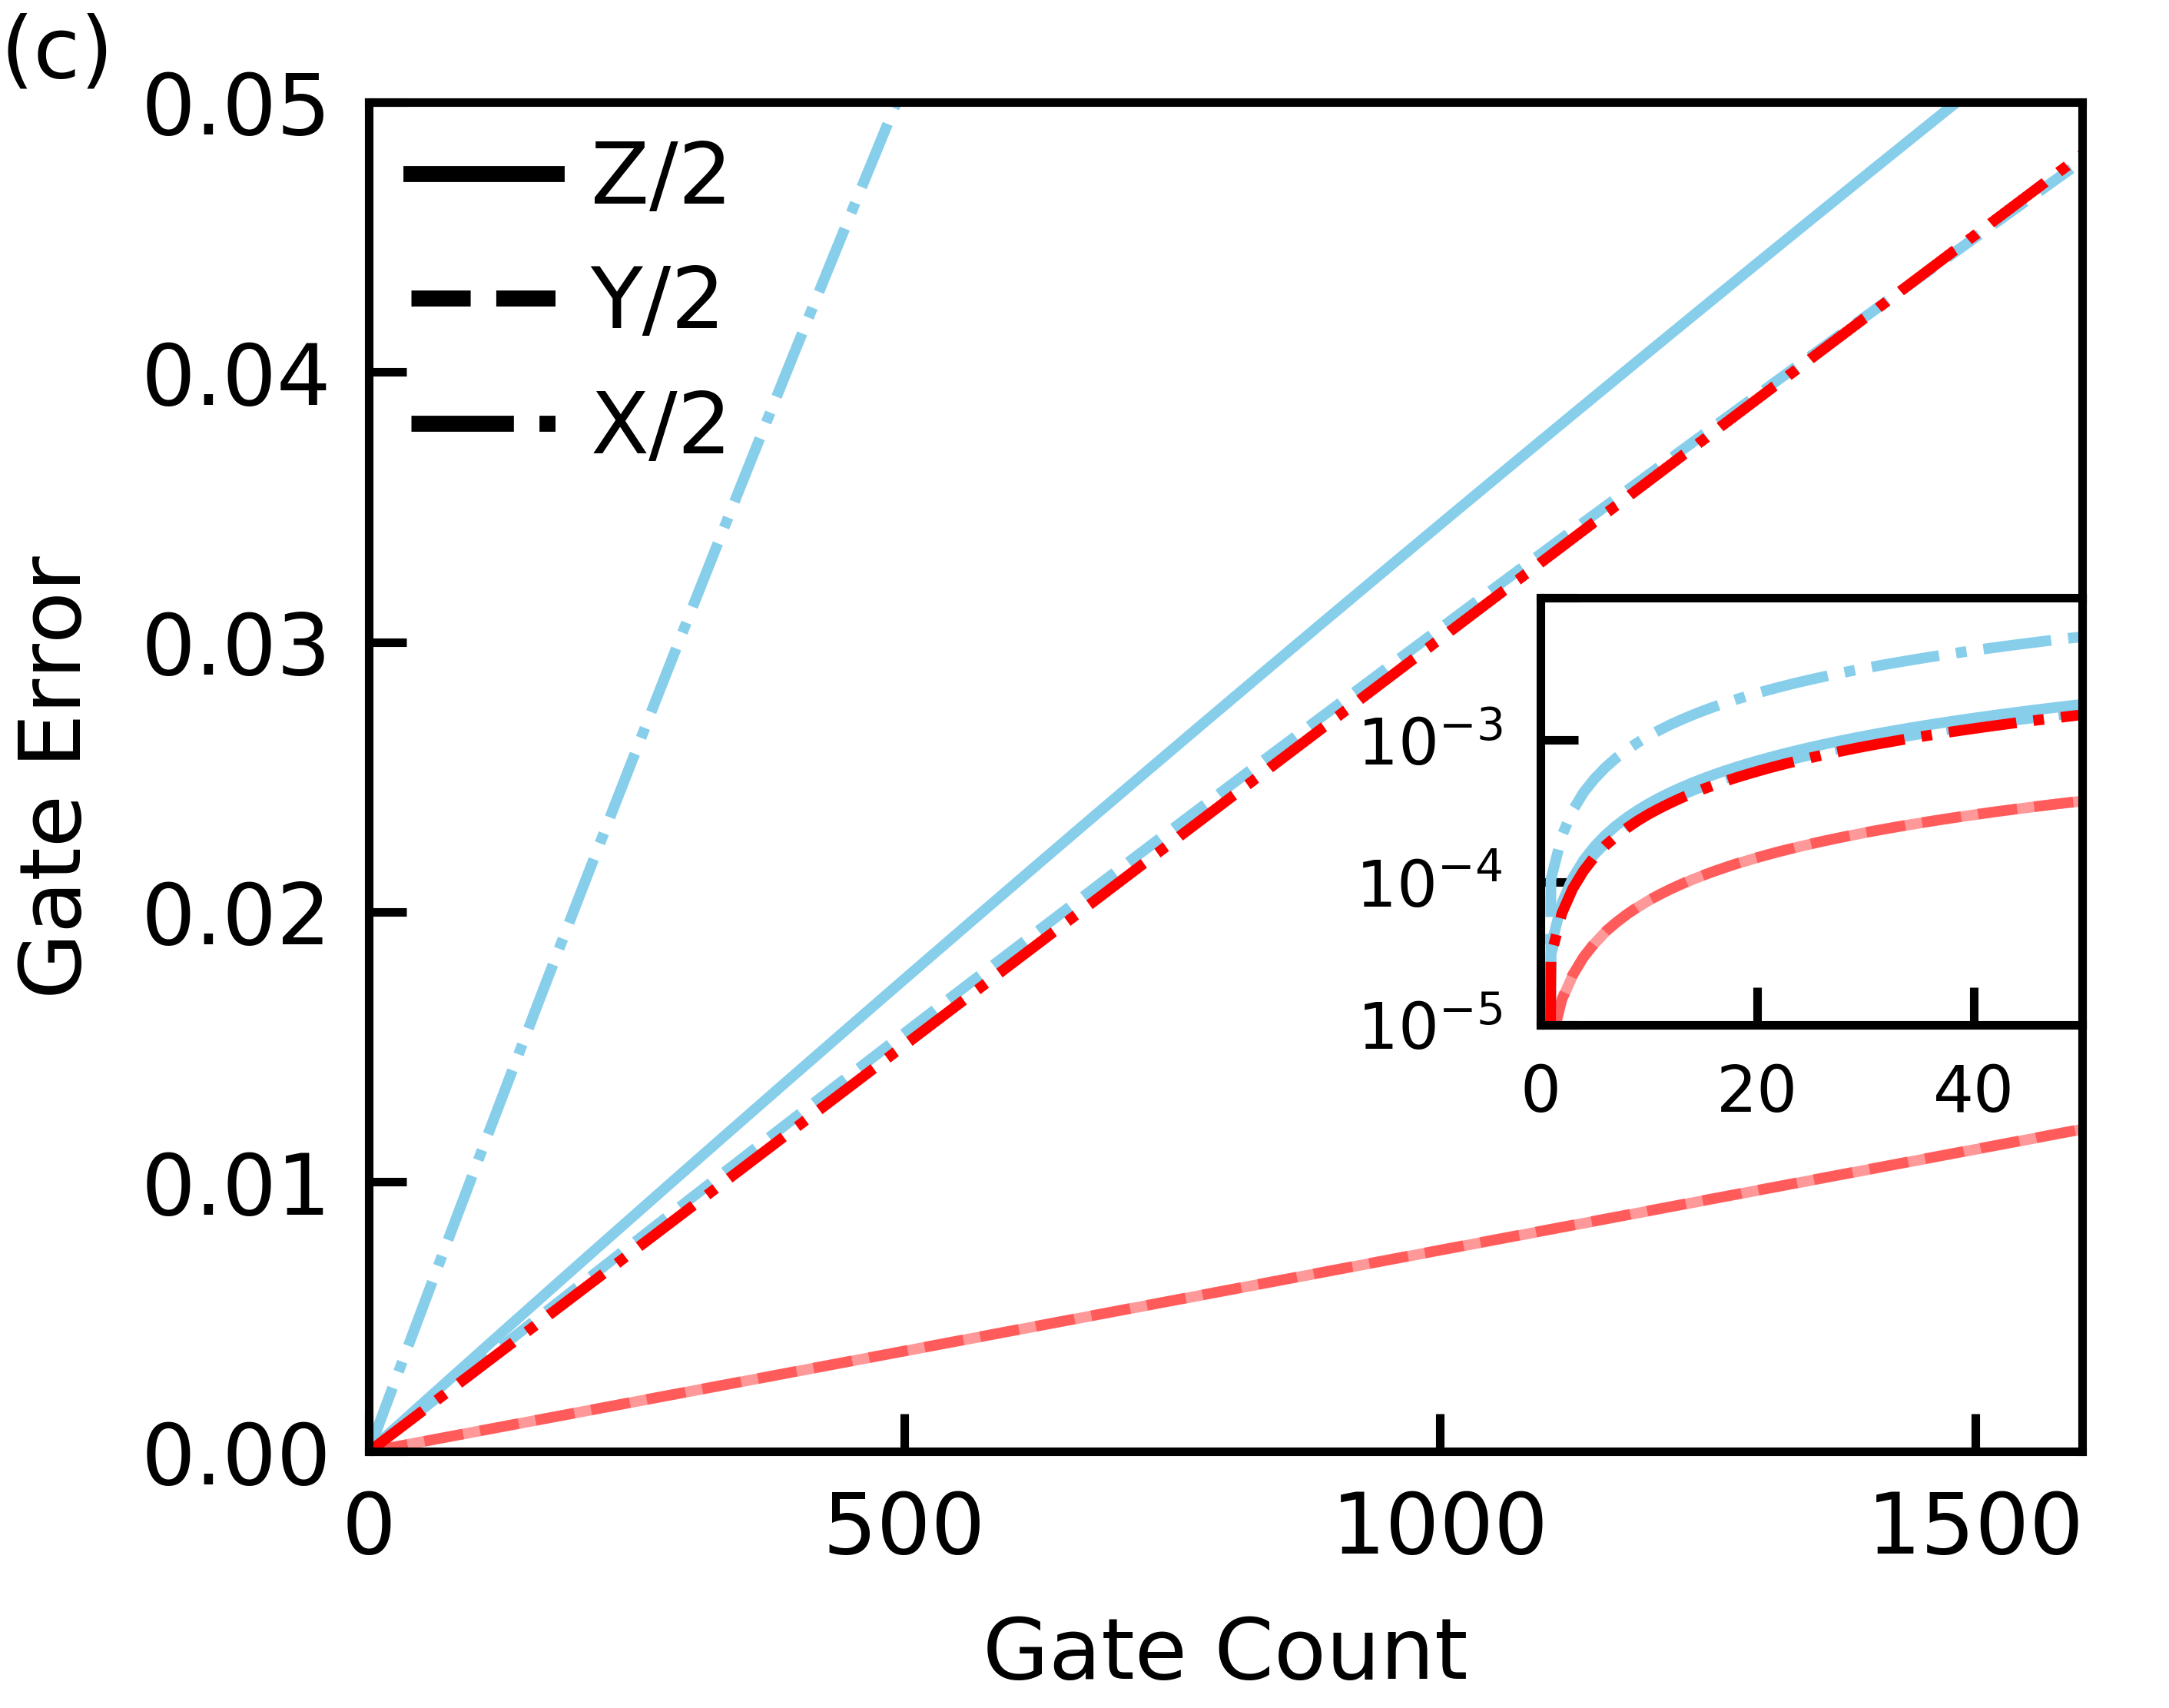
\includegraphics[width=\linewidth]{assets/f1c.png}
  \end{subfigure}
  \caption{
    (a) $T_{1}$ optimized gates (red) and analytic gates (blue).
    (b) $T_{1}$ interpolation function used in optimization. Markers
    denote the time-averaged, absolute amplitude of each gate.
    (c) Lindblad master equation simulation with $T_{1}$ dissipation
    for successive gate applications. The reported gate error is computed after
    each gate appliaction.
  }
\end{figure*}

%% S4
\section{Longitudinal Relaxation Awareness}
(Strategy) We seek to minimize the probability
that the qubit decays as a result of longitudinal
relaxation. To this end we add the
longitudinal relaxation probability
to the augmented state vector
\begin{equation}
  P_{1}(t) = \int_{0}^{t} T_{1}^{-1}(a(t^{\prime})) dt^{\prime}
\end{equation}
Setting the target
longitudinal relaxation probability to 0 results in
a quadratic cost at each knot point
of the form ${\lvert P_{1}(t_{k}) \rvert}^{2}$.

$T_{1}(a_{k})$
is obtained at each knot point by evaluating
a spline interpolant fit to
experimentally obtained data of the form
$\{(a, T_{1})\}$.
Calculating $T_{1}$ directly from theoretical
considerations requires many high-rank
eigendecompositions, which
is computationally expensive. Additionally,
$T_{1}$ values are known to fluctuate greatly
with laboratory temperatures \cite{klimov2018fluctuations}.
Interpolating $T_{1}$ from experimental data increases
the fridge truth of the simulation.

For a given $T_{1}$ time, a shorter gate duration would tend to
favor a lower longitudinal relaxation probability.
We allow the optimizer to tune the gate duration by
making the time step between each knot point $\Delta t_{k}$
a decision variable.
Promoting $\Delta t_{k}$ to a decision variable, rather
than the number of knot points $N$, preserves the
Markovian decision structure of the trajectory
optimization problem. To ensure numerical
integration accuracy is maintained we add a bound
constraint at each knot point
$2.5\textrm{e-}3 \ \textrm{ns} \le
\Delta t_{k} \le 1\textrm{e-}2 \ \textrm{ns}$.
Note that this bound constraint is allowed to be
broken for intermediate iterations of the optimization,
so we add the square root of the time step $\sqrt{\Delta t_{k}}$
to the augmented control vector and use the squared root
of the time step $\lvert \Delta t_{k} \rvert$ in optimization.

(Results) The $Y/2$ and $Z/2$ gates converge on similar solutions, a periodic
waveform with amplitude $\sim 0.2 \textrm{GHz}$ (see Figure 1). Both extend their gate times
beyond their analytic counterpart, trading longer gate times for access
to higher amplitudes and therefore higher $T_{1}$ times. Both gates reduce
their probability of longitudinal relaxation per gate by a factor of $\sim 5$ over
their analytic counterparts. Furthermore, they perform simlarly in
the concatenated gate application comparision, maintaining a total gate error under $10^{-2}$
over $10^{3}$ gate applications, for an average gate error on the order of $10^{-5}$.
We define gate error as the infidelity of the final state and the target state,
averaged over multiple pseudo-randomly
generated initial states. The $X/2$ gate 

%% T1
%% TODO: maybe for appendix.
\begin{table}[ht]
  \begin{tabular}{c | c | c | c}
    & Analytic  & QOC &\\
    Gate & $P_{1}\ (10^{-5})$ & $P_{1}\ (10^{-5})$ & $P_{1\textrm{A}} / P_{1\textrm{Q}}$\\
    \hline
    Z/2 & 5.745 & 1.149 & 5.000\\
    Y/2 & 5.253 & 1.157 & 4.540\\
    X/2 & 16.251 & 4.488 & 3.621\\
  \end{tabular}
  \caption{Probability of longitudinal relaxation for each gate
    evaluated at the gate's duration.}
\end{table}


%% F2
\begin{figure*}[ht]
  \begin{subfigure}{.315\textwidth}
    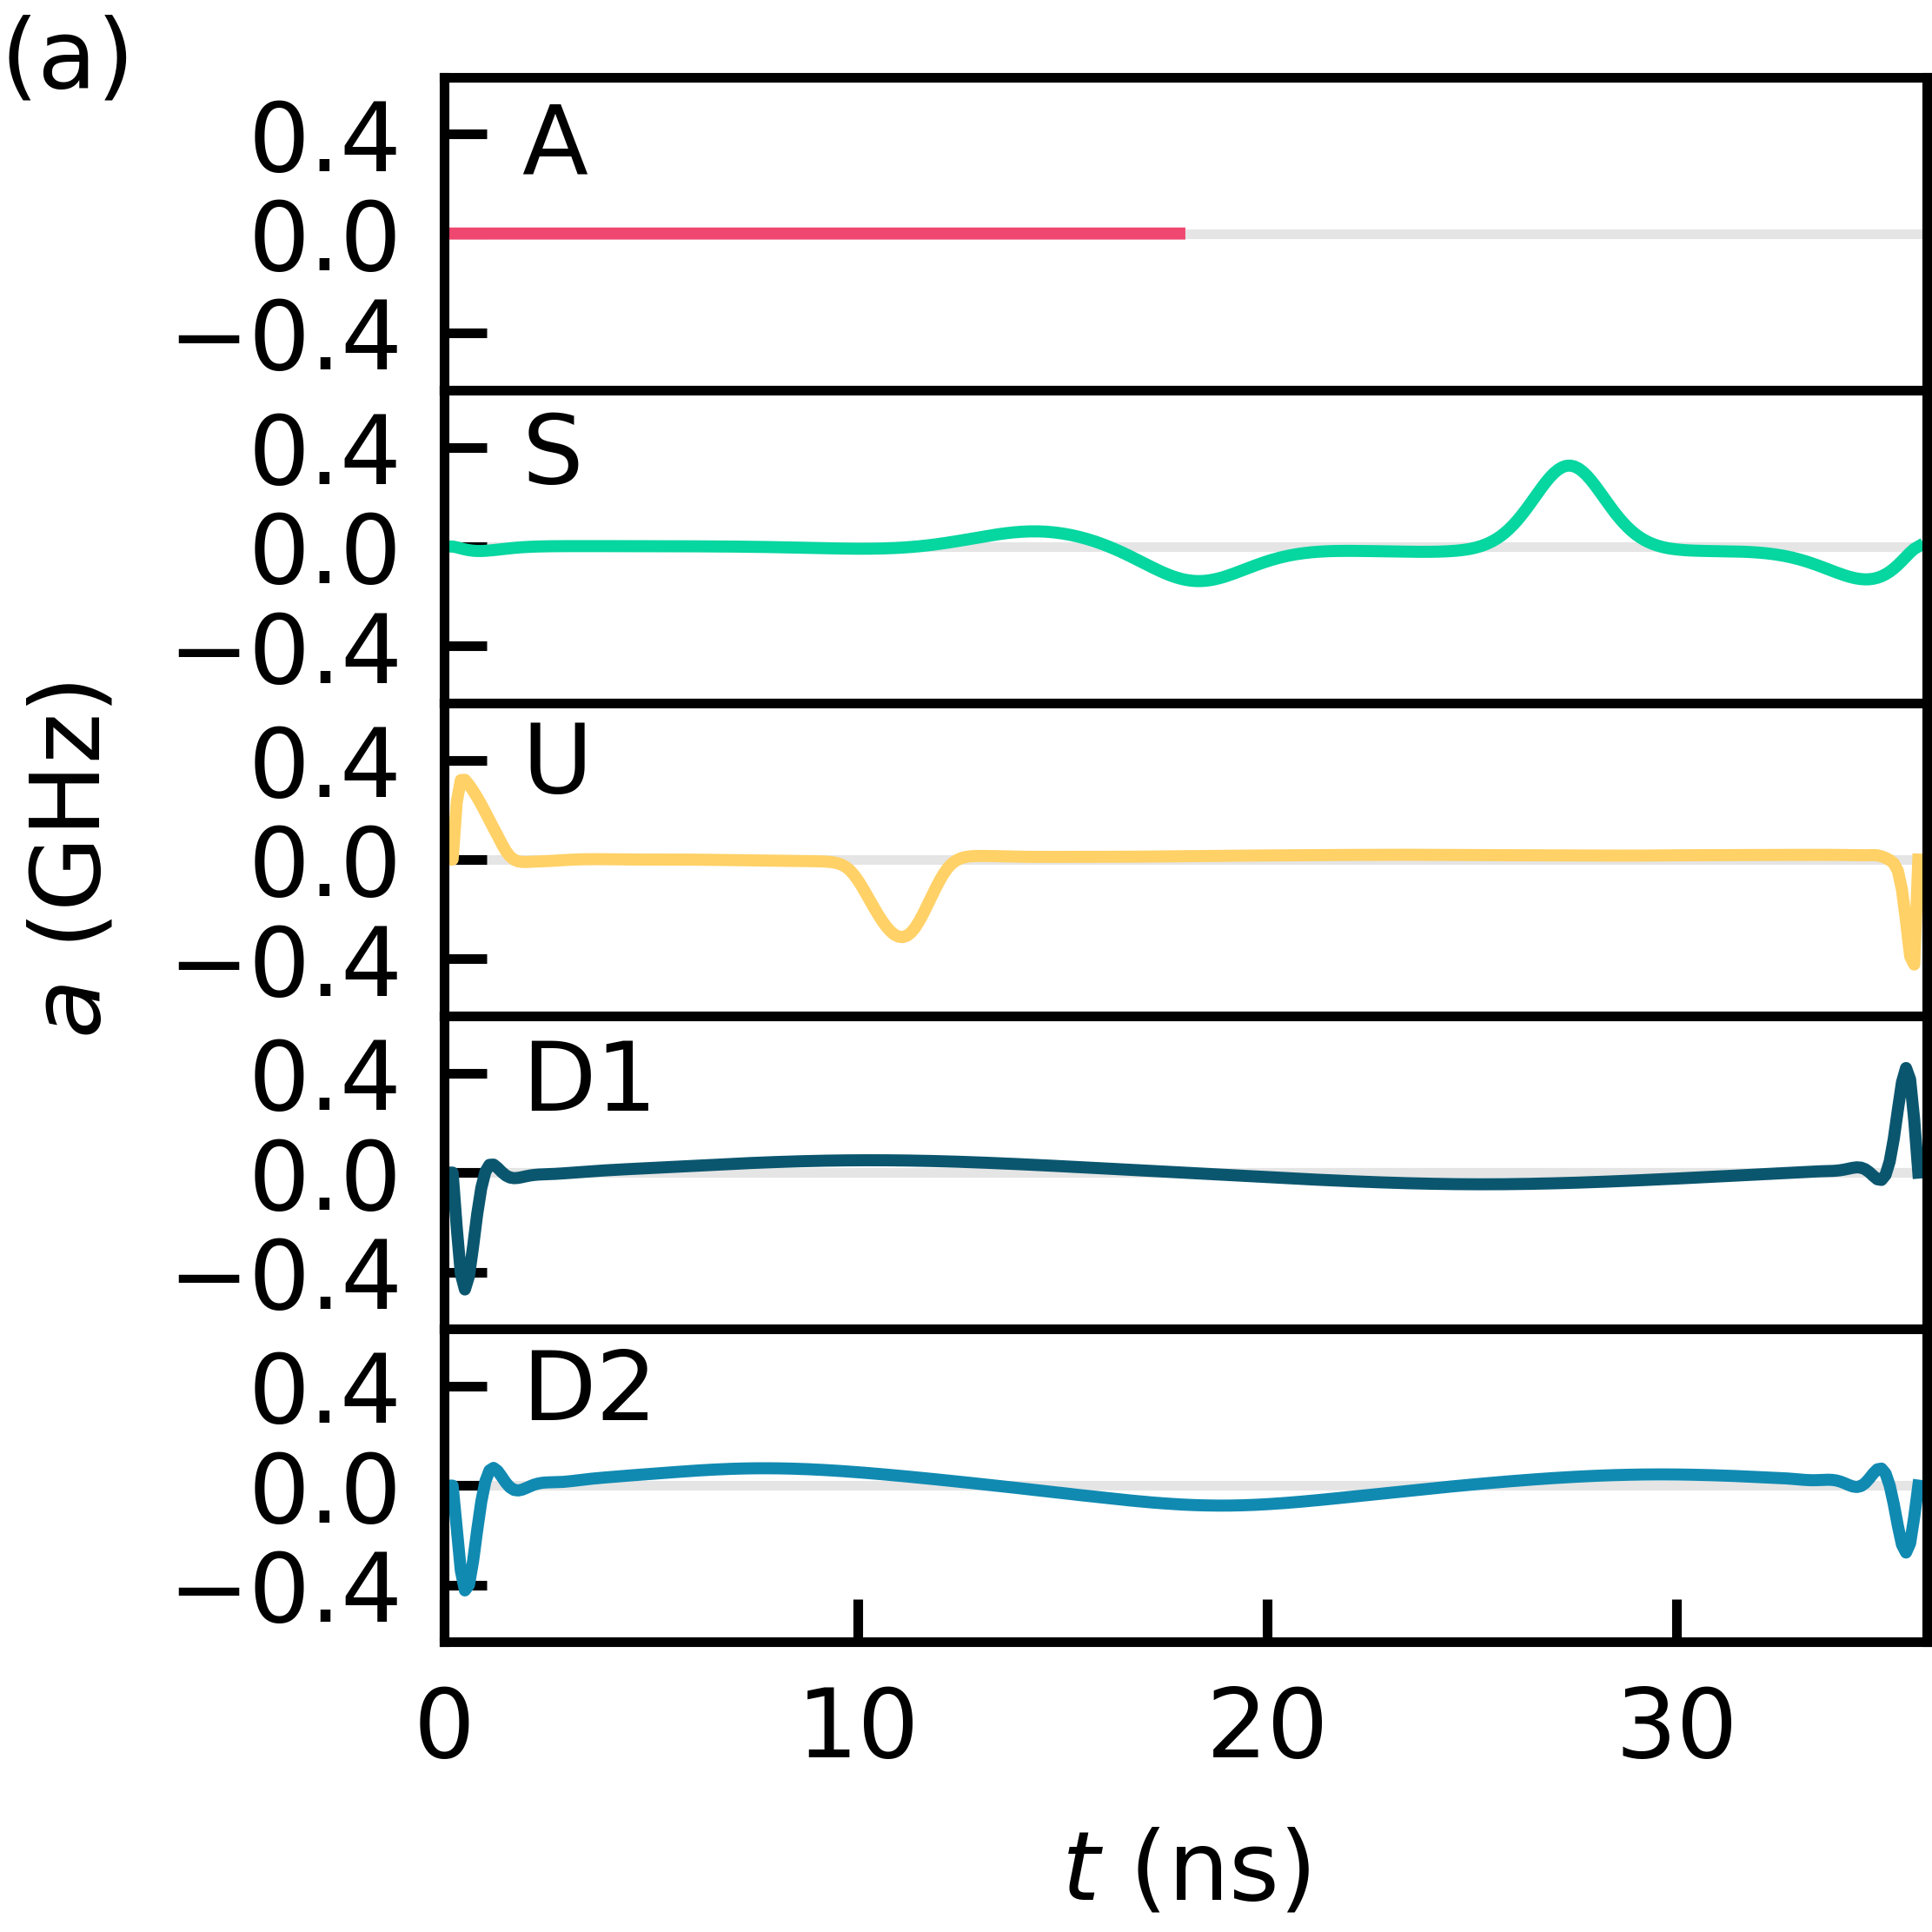
\includegraphics[width=\linewidth]{assets/f2a.png}
  \end{subfigure}\hfill
  \begin{subfigure}{.4\textwidth}
    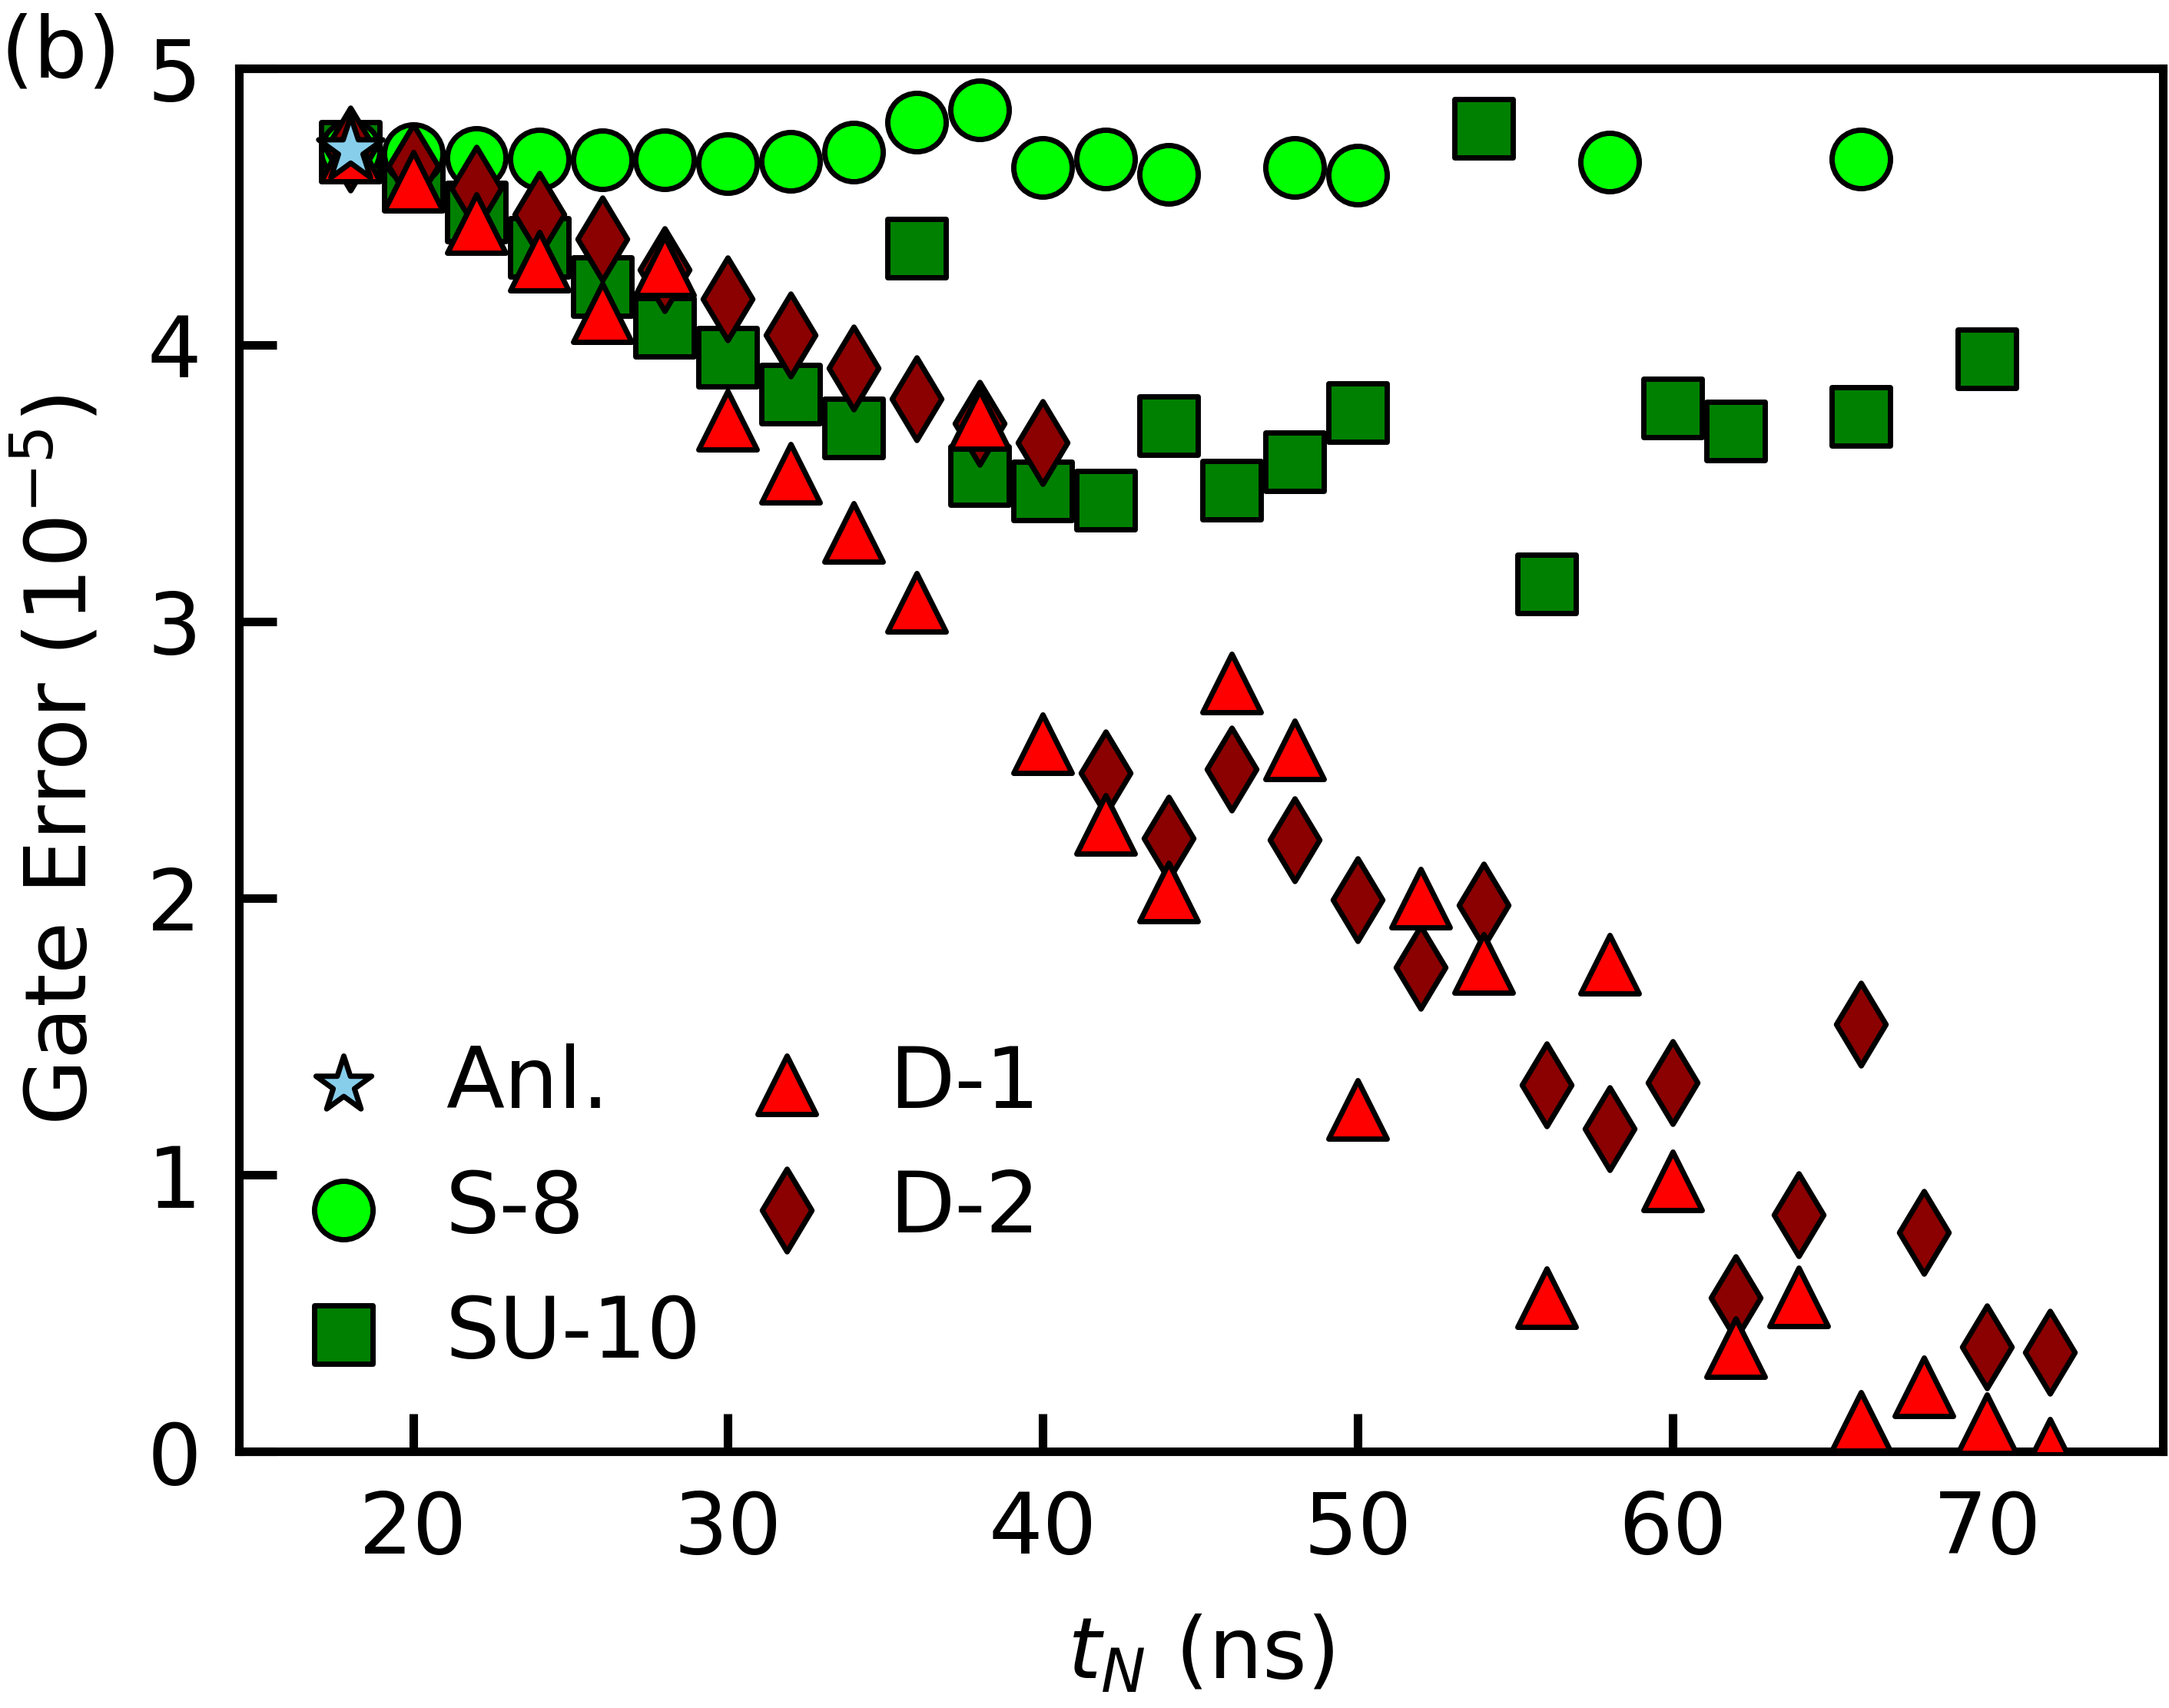
\includegraphics[width=\linewidth]{assets/f2c.png}
  \end{subfigure}\hfill
  \begin{subfigure}{.23\textwidth}
    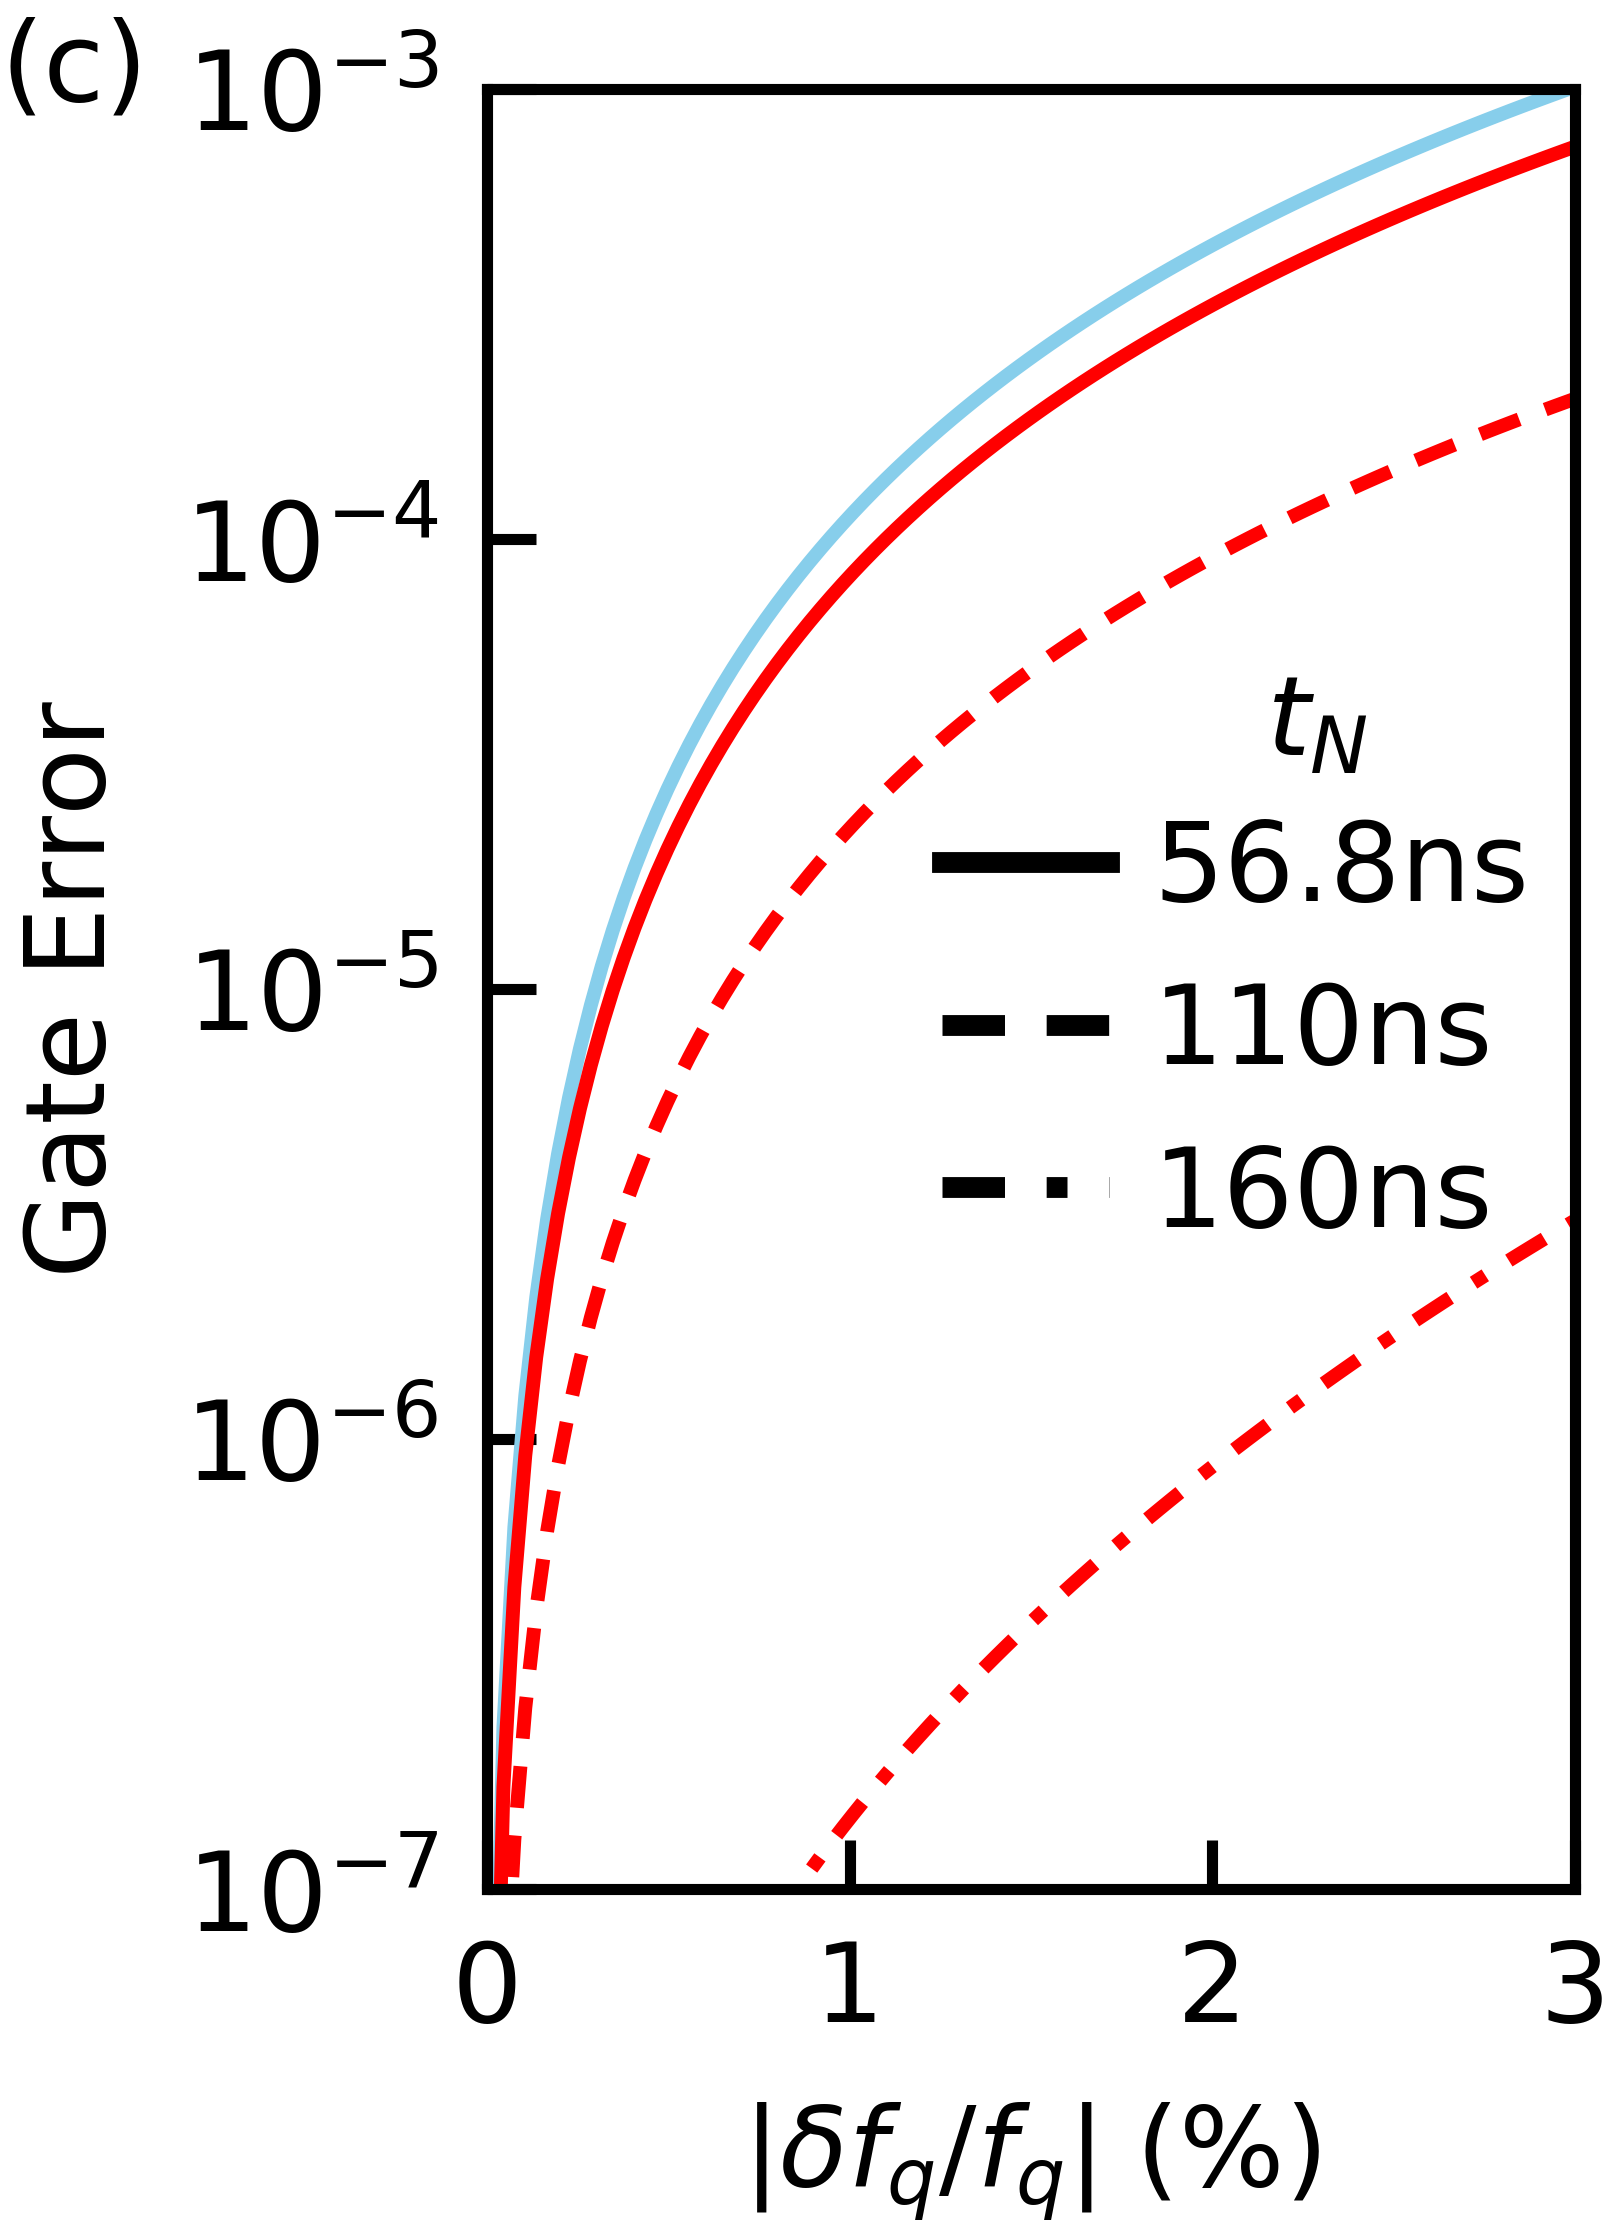
\includegraphics[width=\linewidth]{assets/f2b.png}
  \end{subfigure}
  
  \caption{
    (a) X/2 gates robust to qubit frequency detunings constructed using the
    analytic, 2-point sampling, 8-point unscented sampling, and (2\textsuperscript{nd},
    3\textsuperscript{rd})-order derivative methods at a gate duration of $56.8$ns.
    (b) Single gate error as
    a function of the gate duration at a one-percent
    detuning from the nominal qubit frequency for all methods.
    (c) Single gate error as a function of the detuning from the nominal
    qubit frequency at gate durations of $56.8$ns and $120$ns for the analytic
    and 2\textsuperscript{nd}-order derivative methods.
  }
\end{figure*}

%% F3
\begin{figure}[h]
  \begin{subfigure}{\linewidth}
    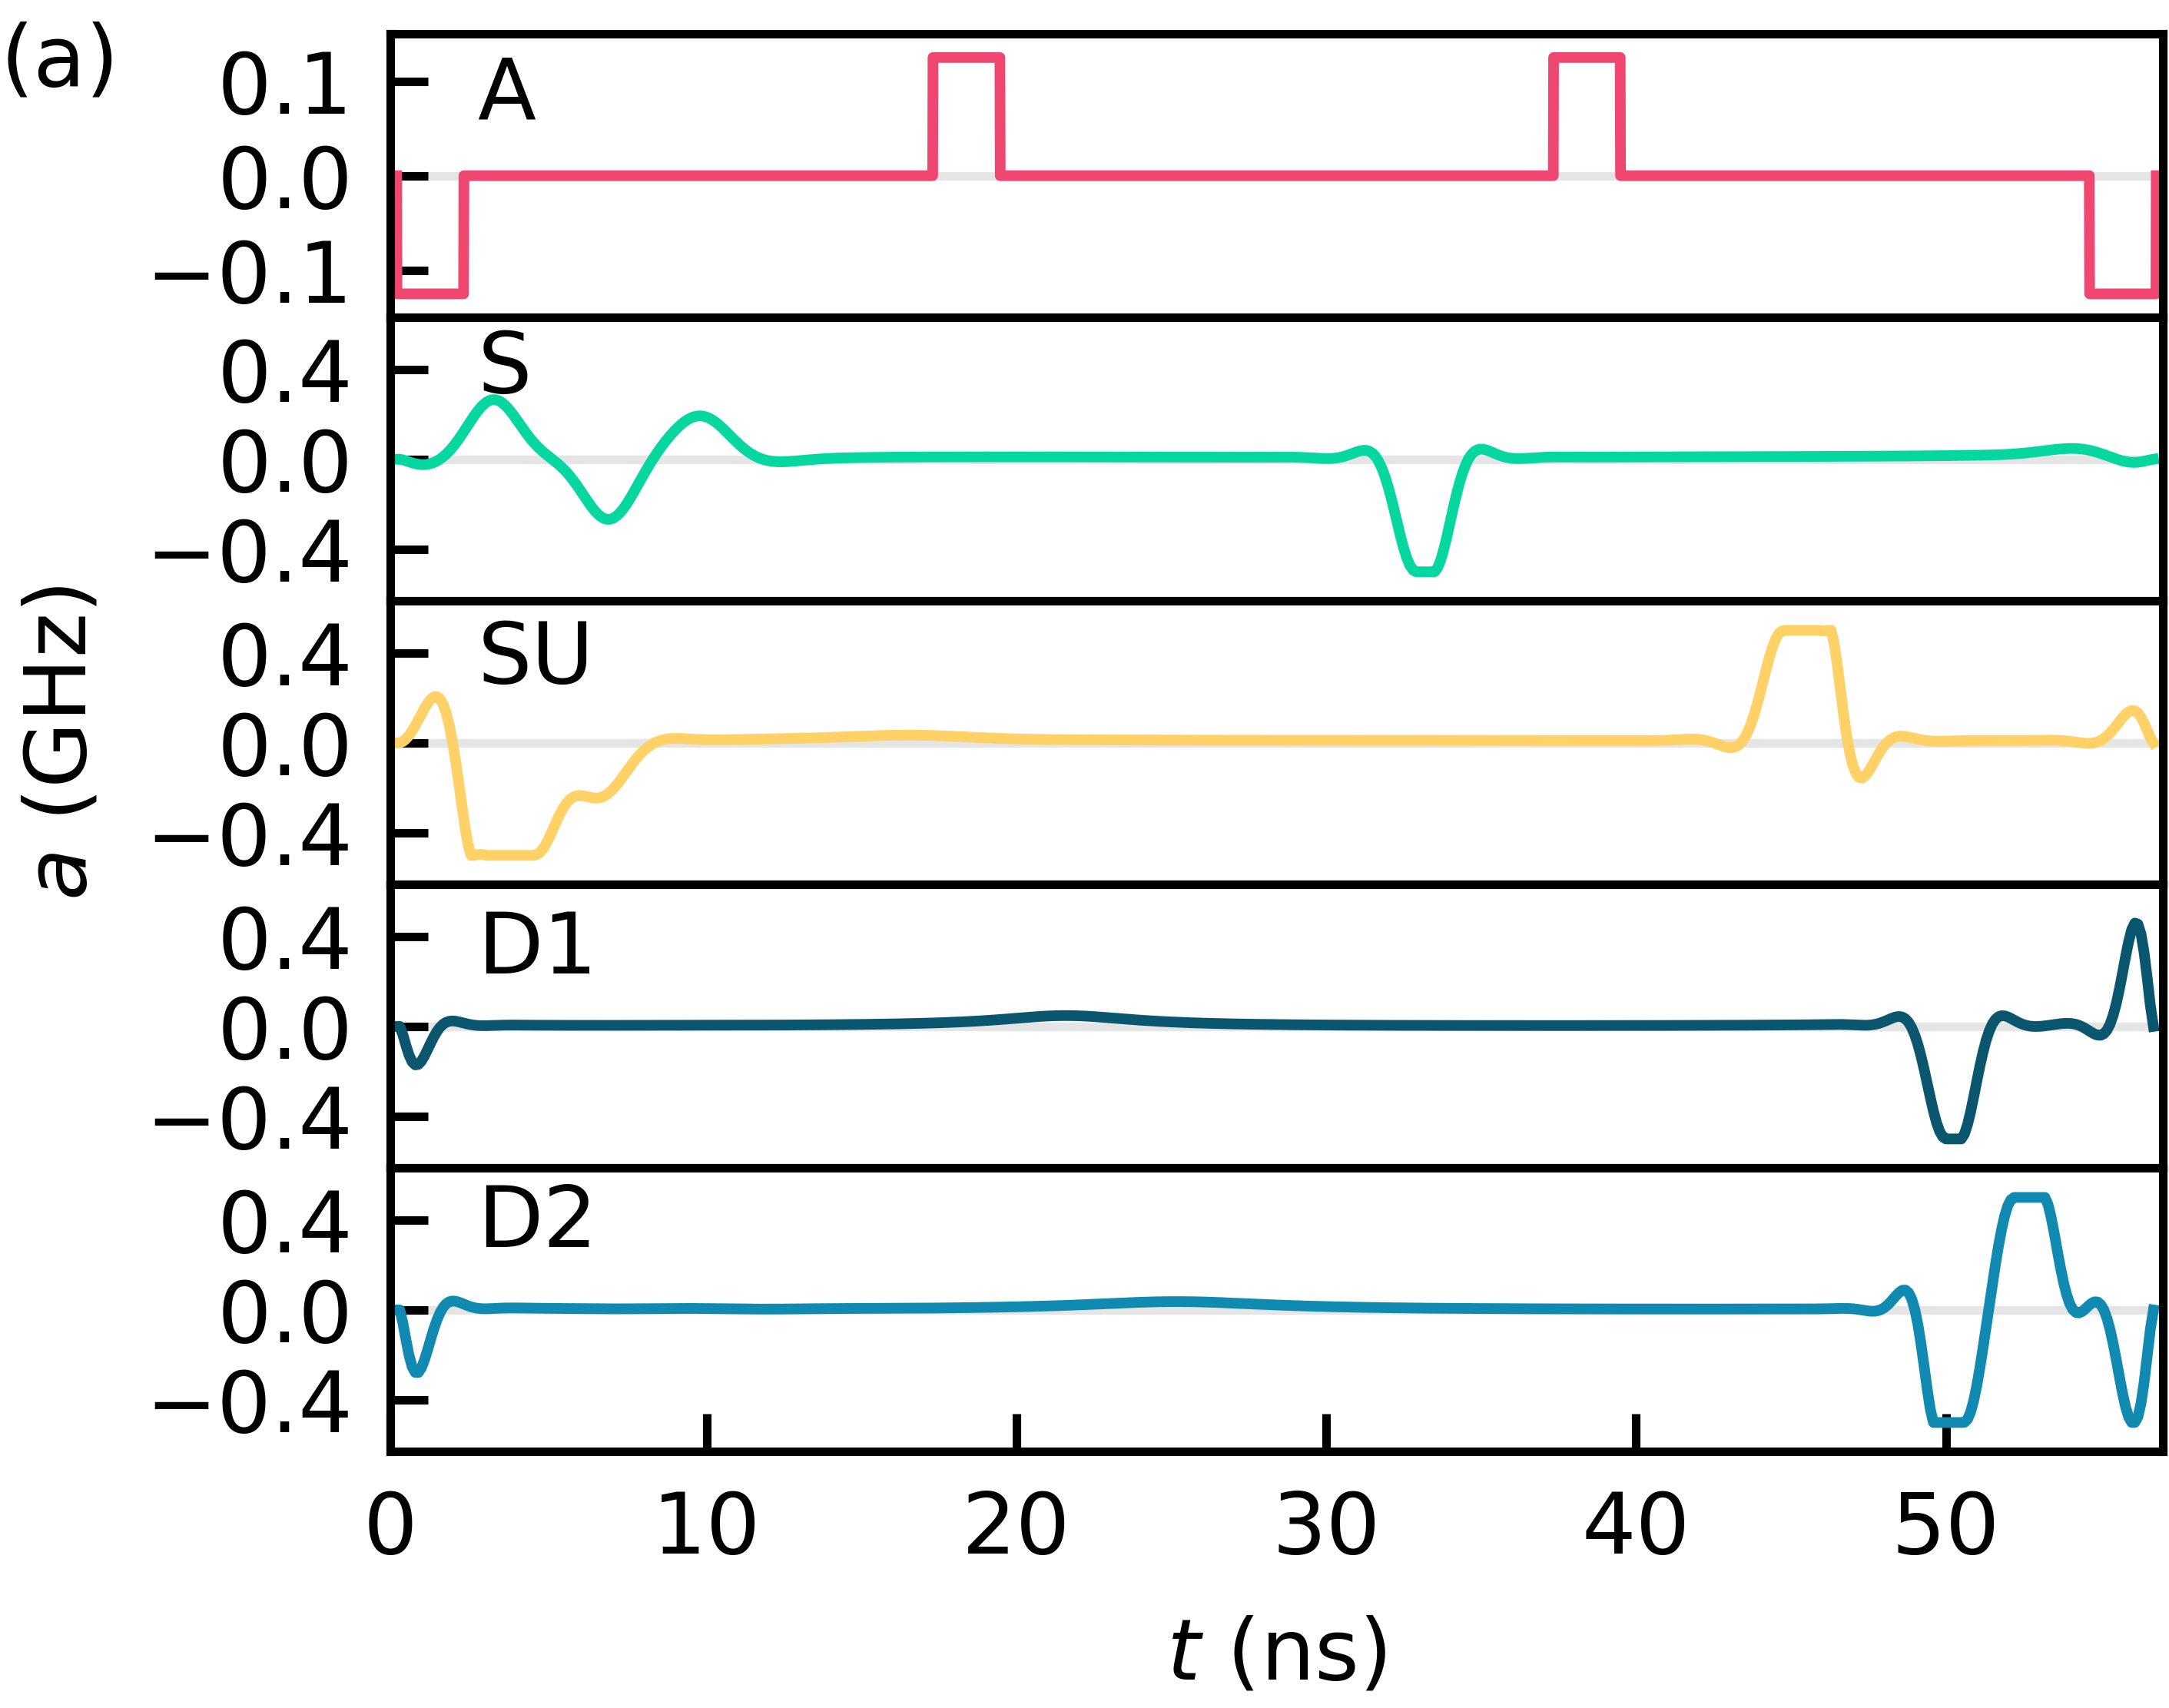
\includegraphics[width=\linewidth]{assets/f3a.png}
  \end{subfigure}
  
  \begin{subfigure}{\linewidth}
    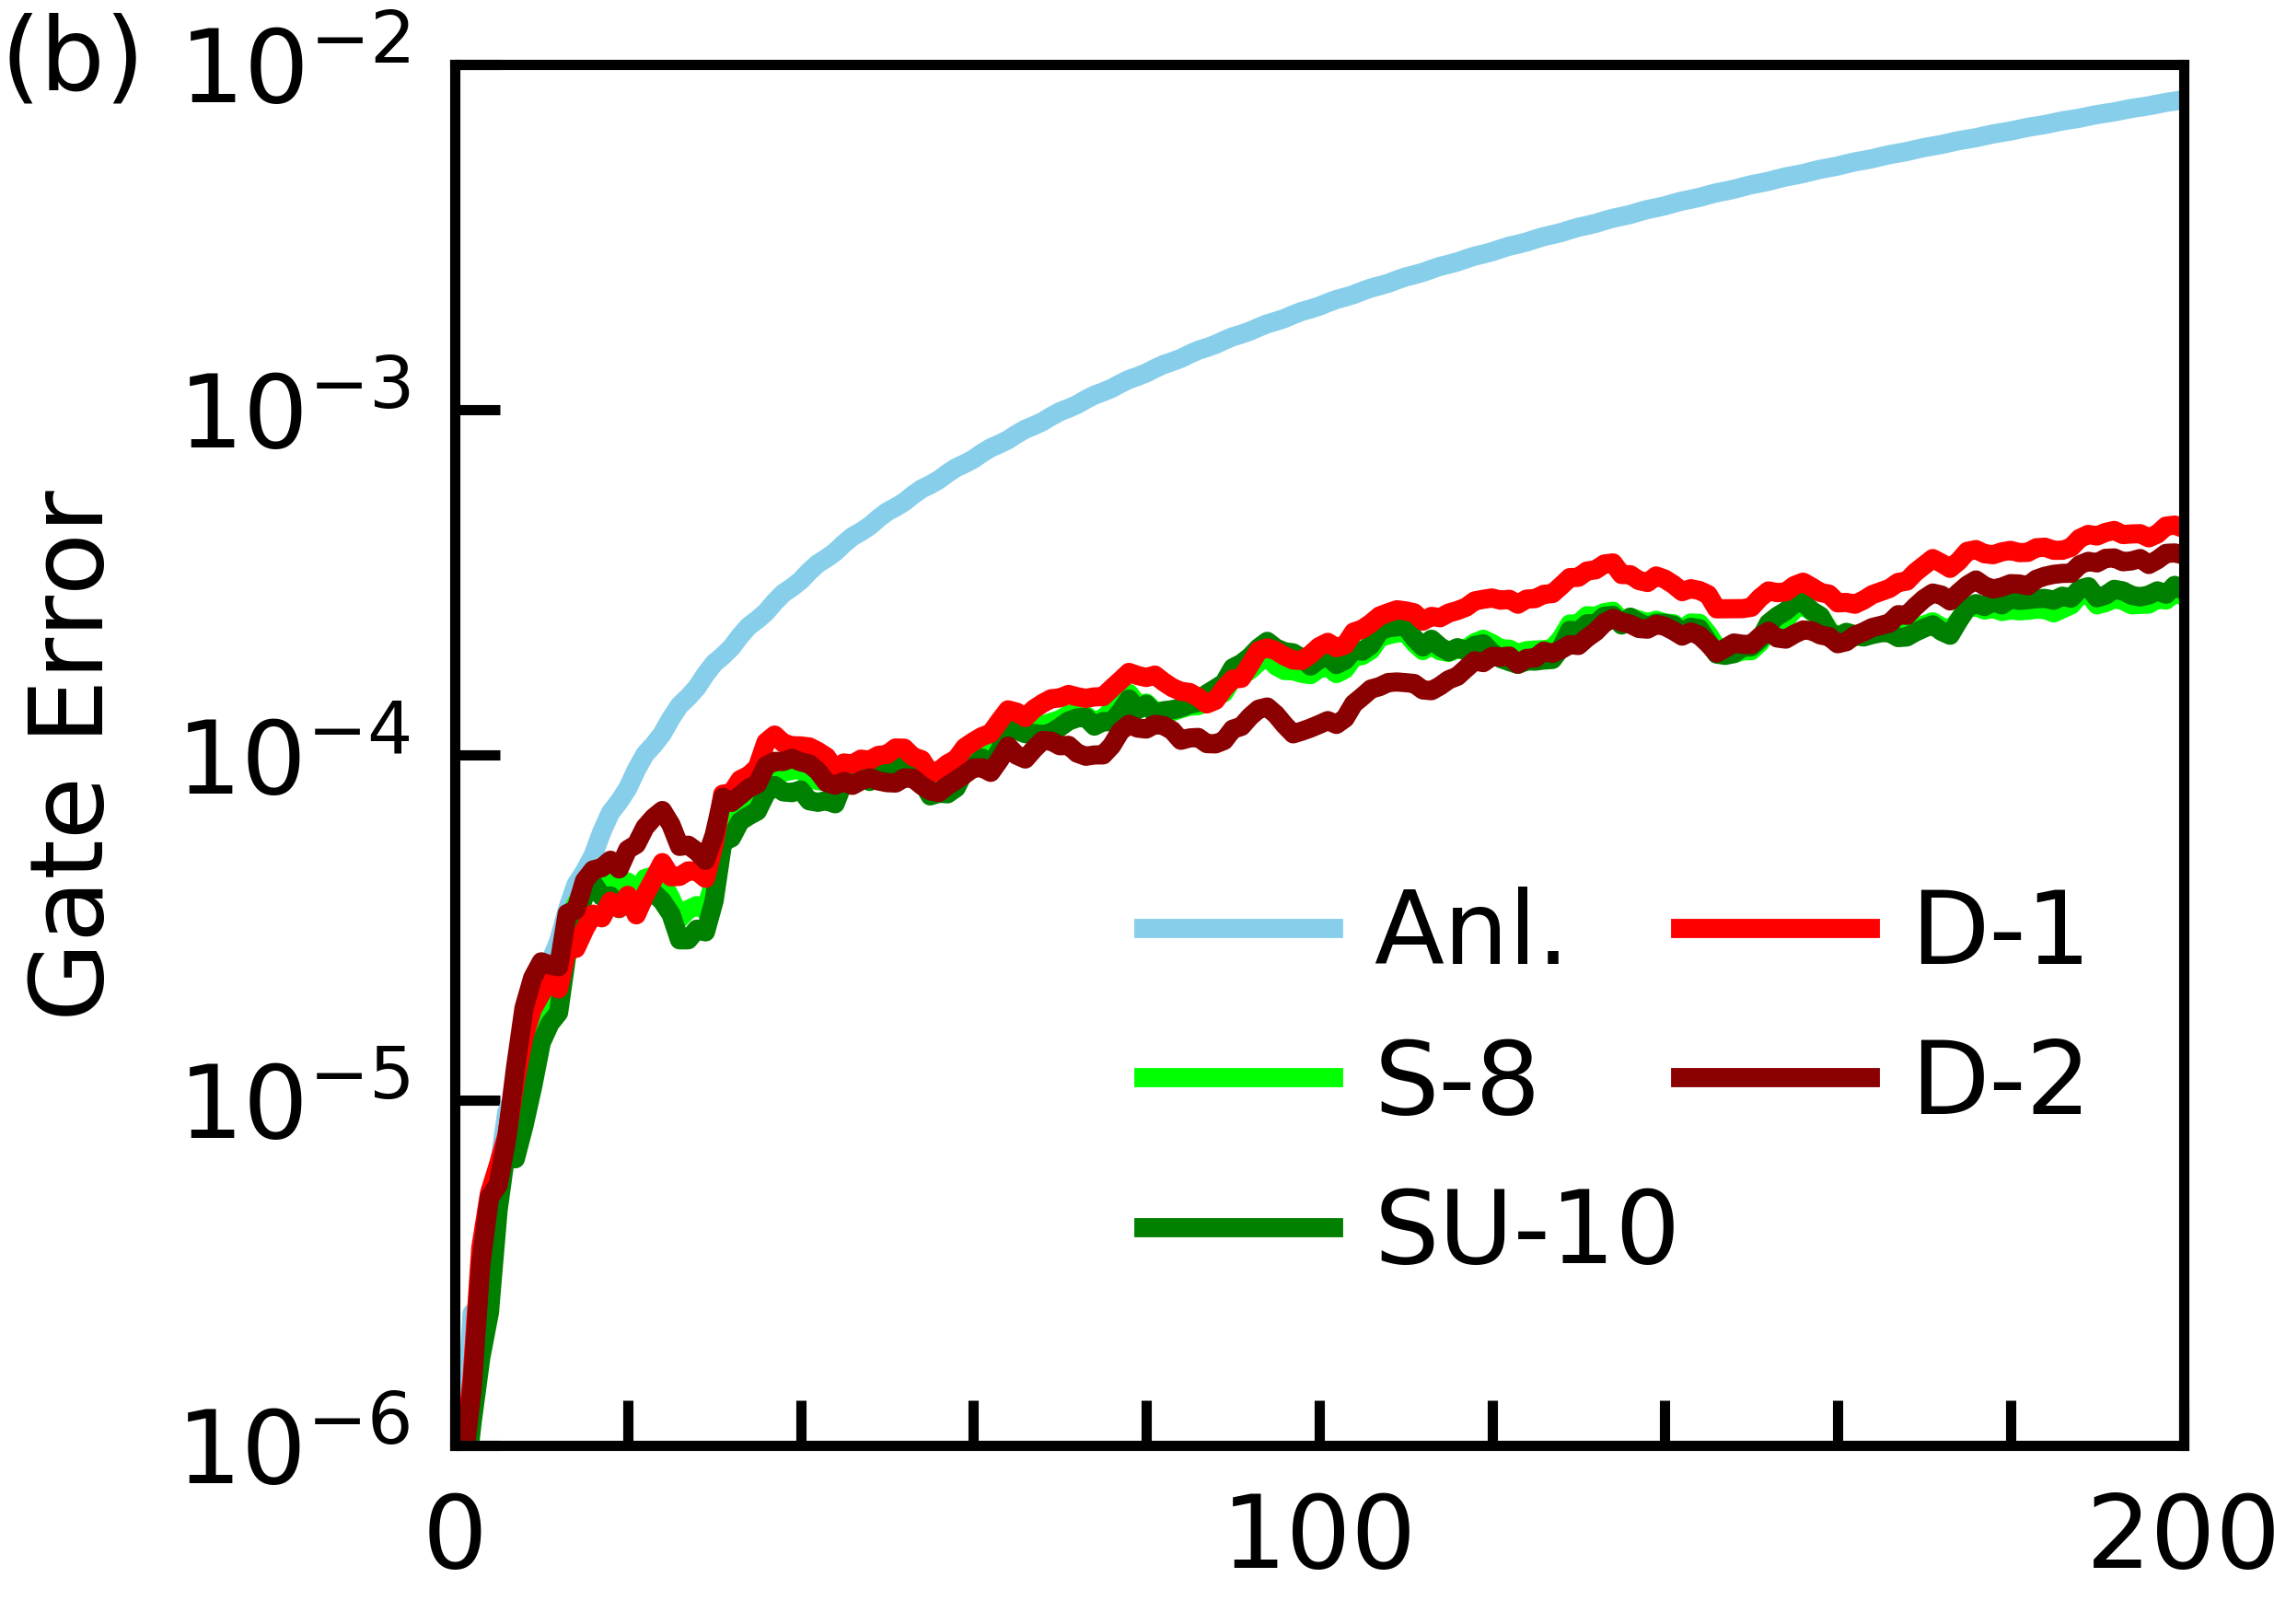
\includegraphics[width=\linewidth]{assets/f3b.png}
  \end{subfigure}

  \caption{
    (a) $X/2$ gates robust to flux offsets constructed using the analytic,
    (2, 4)-point sampling, and (2\textsuperscript{nd}, 3\textsuperscript{rd})-order
    derivative methods at a gate duration
    of $56.8$ns. (b) Simulation of stochastic 1/$f$ flux noise for
    successive gate applications. The reported gate error is measured
    after each gate application.
  }
\end{figure}

%% S5
\section{Robustness to Parameter Deviations}
(Strategy) Magentic flux noise,
Johnson-Nyquist current noise present in the flux bias
lines, and temperature dependent gain fluctuations
may cause the flux amplitude to deviate from its
desired value by an amount $\delta a$. Additionally,
residual calibration errors and fluctuations may cause
the qubit frequency to deviate from its measured value
by an amount $\delta f_{q}$.

System parameter
deviations are typically addressed with dynamic decoupling
sequences \cite{merrill2014progress},
the DRAG scheme \cite{krantz2019quantum}, or
geometric phase considerations
\cite{xu2020nonadiabatic} \cite{han2020experimental}.
Dynamic decoupling sequences compose rotations on the
Bloch sphere so that erroneous rotations arising due
to the parameter deviation are cancelled.
%% The latter two methods are inflexible.
We draw on the
robust control literature to demonstrate
numerical techniques for engineering robustness
to parameter deviations.

We propose two methods for engineering robustness
to parameter deviations. The first is the
derivative method. We draw on the intuition that
the sensitivity of the state evolution to the parameter
$\lambda$ is encoded in the derivative of
the state with respect to that parameter
$\partial_{\lambda}^{l} \ket{\psi}$. The derivative
scheme aims to minimize the norm of this derivative.
The derviatives of the state with respect to the parameter
of interest are propgated in the
augmented state vector. Their dynamics are found by differentiating
the TDSE dynamics with respect to the parameter of interest
(see Appendix). Setting the target derivatives of the state
to the zero vector results in quadratic costs at each
knot point
${\lvert \partial_{\lambda}^{l} \ket{\psi} \rvert}^{2}$.
In the $l$\textsuperscript{th}-order derivative method, the norm of
all derivatives of order less than or equal to $l$ are penalized. For example,
in the 2\textsuperscript{nd}-order derivative method both the
1\textsuperscript{st}-order state derivative
(${\lvert \partial_{\lambda} \ket{\psi_{k}} \rvert}^{2}$)
and the 2\textsuperscript{nd}-order state derivative
(${\lvert \partial^{2}_{\lambda} \ket{\psi_{k}} \rvert}^{2}$)
contribute quadratic costs at each knot point.

The second scheme we analyze is the sampling method,
which is well studied in the robust control literature
\cite{manchester2016derivative} \cite{tronarp2016sigma}.
We add additional
states to the augmented state vector that follow deviant dynamics, and
penalize the state's difference from the target state.
The deviant dynamics are given by the system
Hamiltonian with the parameter of interest replaced by
a deviant value $\lambda \gets \lambda + \delta \lambda$
The parameter's deviation is typically chosen
to represent the statistical distribution of the parameter.
For example, in the 2-point sampling method we
propagate the additional states $\ket{\psi^{\pm}}$ where
$\lambda^{\pm} = \lambda \pm \sigma_{\lambda}$, with
$\sigma_{\lambda}$ being the standard deviation of $\lambda$.
The difference between the final states and the target
state is penalized, resulting in quadratic costs at
each knot point
${\lvert \ket{\psi^{\pm}_{k}} - \ket{\psi_{f}} \rvert}^{2}$.
For the 4-point sampling method we sample at two standard deviations
above and below the nominal parameter value in addition to one standard
deviation above and below.

(Comparison) To demonstrate the applicability of these techniques
to mitigate system parameter deviations,
we consider the task of achieving a single $X/2$
gate subject to a constant qubit frequency detuning
($f_{q} \gets f_{q} + \delta f_{q}$).
%% We use a compensating for off-resonance error
%% (CORPSE) dynamic decoupling pulse that is optimized
%% to mitigate first-order error arising due to the detuning.
%% The pulse is composed of
%% three rotations about the $\hat{x}$, $-\hat{x}$, and $\hat{x}$ axes
%% of the Bloch sphere
%% designed to compensate for erroneous rotations
%% (see Appendix).
We take $\sigma_{f_{q}} = 1\% f_{q}$ to be one standard devation, and equip
the sampling robustness methods accordingly.
For each method we compute the gate error for one simulated gate application
subject to the stated deviant dynamics.

(Results) Both the 2-point and 4-point
sampling methods converge on a similar solution with a low amplitude and
a single amplitude parity switch (see Figure 2a). At the gate time of the analytic pulse
($56.8$ ns) and a one percent qubit frequency detuning they achieve
gate errors $\sim 1.1 \cdot 10^{-4}$ commensurate with the analytic
pulse $\sim 1.2 \cdot 10^{-4}$. The 2-point and 4-point sampling methods
achieve similar metrics in simulation (see Table 2).

Both the 2\textsuperscript{nd}-order and 3\textsuperscript{rd}-order derivative methods
employ multiple amplitude parity switches and idle periods at the maximum
amplitude $0.5$ GHz. At the gate time of the analytic pulse and a one percent qubit
frequency detuning, the 2\textsuperscript{nd}-order method achieves a gate error
$\sim 0.8 \cdot 10^{-4}$ and the 3\textsuperscript{rd}-order method achieves a gate error
$\sim 1.1 \cdot 10^{-4}$ (see Figure 2b). Inspection of the simulation metrics reveals
that the 3\textsuperscript{rd}-order method is able to achieve a lower norm of the
3\textsuperscript{rd}-order state derivative at the cost of higher 1\textsuperscript{st}-order
and 2\textsuperscript{nd}-order derivatives than the 2\textsuperscript{nd}-order method (see Table 3).

%% T2
\begin{table}
  \begin{tabular}{c | c | c | c}
    Method & ${\lvert \partial_{f_{q}} \ket{\psi} \rvert}^{2}$ ($10^{3}$)
    & ${\lvert \partial^{2}_{f_{q}} \ket{\psi} \rvert}^{2}$ ($10^{7}$)
    & ${\lvert \partial^{3}_{f_{q}} \ket{\psi} \rvert}^{2}$ ($10^{12}$)\\
    \hline
    D-2 & 8.706 & 8.331 & 3.692\\
    D-3 & 9.643 & 9.095 & 3.345\\
  \end{tabular}
  \caption{Norm of basis state derivatives undergoing a $X/2$ gate for the derivative methods at $t_{N} = 56.8$ns}
\end{table}

Further, we observe that the derivative methods are able
to take advantage of an increased gate duration to achieve greater robustness,
while the sampling methods are unable to. The tradeoff between gate error and
gate duration appears roughly linear, where trading 3 times the gate duration
results in a factor of 4 reduction in gate error for the 2\textsuperscript{nd}-order
derivative method (using the 50ns and 150ns points, include this remark?). Additionally,
no optimization converged for gate durations less than 50ns., and robustness commensurate
with the analytic pulse at a shorter gate duration was not able to be achieved.


%% TODO: maybe add new section
(Comparison) An additional task of interest is to mitigate
stochastic parameter deviations. For the fluxonium qubit, magnetic flux noise
acts to modify the flux amplitude from its intended value by an amount $\delta a$.
It is well studied that the spectral density of $\delta a$ follows a
1/$f$ distribution, consisting primarily of low frequency noise. We compare
the methods discussed for static parameter deviations to the task of
realizing a $X/2$ gate subject to 1/$f$ flux noise. We simulate successive
applications of the gate constructed by each method and measure the gate error
after each application (see Figure 3b). The system is subject to flux noise
$\delta a (t)$ that is generated from a standard normal distribution, normalized
by 1/$f^{1/2}$ in frequency space, and modulated by the experimentally obtained
flux noise amplitude $A_{\Phi} = 5.21 \mu \Phi_{0}$.

(Results) ...


%% S6
\section{Conclusion}
We have proposed some schemes and they work well.


%% ACK
\begin{acknowledgments}
  The authors would like to thank Helin Zhang for experimental assistance,
  and Stephen Lyon (maybe) and Daniel Weiss for useful discussions.
\end{acknowledgments}


\appendix
%% AA
\section{Ricatti Recursion}
This will give the reader unfamiliar with trajectory
optimization intuition for how the trajectory optimization
update scheme works and why it is better than
a more naive method.


%% AB
\section{Experiment}
We measure $T_{1}$ using the standard experiment
and $T_{2}$ using te Ramsey experiment. We fit with splines
and the data looks like fig. 3 in Helin's paper \cite{zhang2020universal}.
We measure $f_{q}$ and $\sigma_{f_{q}}$ using X method.


%% AC
\section{Dissipation Simulation}
We model dissipation using the Lindblad master
equation. 
\begin{equation}
  \frac{d}{dt} \rho = \frac{-i}{\hbar} [H, \rho] + \sum_{i = 1}^{N^{2} - 1} \gamma_{i} (L_{i} \rho L_{i}^{\dagger} - \frac{1}{2} \{L_{i}^{\dagger} L_{i}, \rho\})
\end{equation}
where $\rho = \ket{\psi}\bra{\psi}$ is the density matrix, $N = \textrm{dim}(\mathcal{H})$,
and $[\cdot, \cdot], \{\cdot, \cdot \}$ are the algebraic commutator and anti-commutator.
For longitudinal relaxation $\gamma_{1} = T_{1}^{-1} = T_{1, \uparrow}^{-1} + T_{1, \downarrow}^{-1}$
and $L_{\uparrow} = \sigma^{+}/2$,
$L_{\downarrow} = \sigma^{-}/2$
are the ladder operators $\sigma^{\pm} = \sigma_{x} \pm i \sigma_{y}$. For pure dephasing
$\gamma_{2} = T_{2}^{-1} = (2 T_{1})^{-1} + T_{\phi}^{-1}$ and
$L_{2} = (I - \sigma_{z})/2$.


%% AD
\section{Derivative Method Dynamics}
To obtain the dynamics for the derivative of the state $\partial_{x}^{l} \ket{\psi(t)}$
we differentiate the TDSE dynamics \ref{eq:tdse} with respect to the parameter of interest
($x$). Using the fluxonium hamiltonian \ref{eq:hamiltonian} we obtain the derivative of the
state with respect to the qubit frequency ($f_{q}$) and the flux amplitude ($a$).
Here we present the dynamics for the second derivative of the state with respect to the
qubit frequency. The case is analogous for the flux amplitude. Both $H$ and $\ket{\psi}$ are functions
of $f_{q}$, $a$, and $t$, but we omit the explicit dependence in notation for
brevity.
\begin{equation}
  \begin{aligned}
      \partial_{f_{q}} \partial_{t} \ket{\psi} &= \partial_{f_{q}} H \ket{\psi}\\
      &= (\partial_{f_{q}} H) \ket{\psi} + H (\partial_{f_{q}} \ket{\psi})\\
      &= \frac{\sigma_{z}}{2} \ket{\psi} + H (\partial_{f_{q}} \ket{\psi})
  \end{aligned}
\end{equation}
\begin{equation}
  \begin{aligned}
    \partial_{f_{q}}^{2} \partial_{t} \ket{\psi} &= \partial_{f_{q}} (\partial_{f_{q}} H \ket{\psi})\\
    &= (\partial_{f_{q}}^{2} H) \ket{\psi} + 2 (\partial_{f_{q}} H)(\partial_{f_{q}} \ket{\psi})\\
    &\quad + H (\partial_{f_{q}}^{2} \ket{\psi})\\
    &= \sigma_{z} (\partial_{f_{q}} \ket{\psi}) + H (\partial_{f_{q}}^{2} \ket{\psi})
  \end{aligned}
\end{equation}
The augmented state vector carries $\partial_{f_{q}}^{l} \ket{\psi}$
which appears explicitly in its own dynamics. Due to the dependence of $H$ on $f_{q}$ and $a$,
the $l$\textsuperscript{th} state derivative is coupled to the
$l - 1$\textsuperscript{th} state derivative.


%% AE
\section{Dynamic Decoupling Sequences}
Here we present the equations for constructing the CORPSE and
B2CORPSE sequences.


%% AF
\section{Complex Tensor Handling}
We use an isomorphism $\mathcal{H}(\mathbb{C}^{n}) \cong \mathcal{H}(\mathbb{R}^{2n})$
because the software we use does not support complex numbers yet.


\bibliography{refs}

\end{document}
